\documentclass[a4paper]{article}

\usepackage[T1]{fontenc}
\usepackage[utf8]{inputenc}
\usepackage[english]{babel}
\usepackage{csquotes}
\usepackage{listings}
\usepackage{multicol}
\lstset{language=c,frame=single,captionpos=b}
\usepackage{hyperref}
\usepackage{amsmath}
\usepackage[backend=biber, sorting=none,maxbibnames=40]{biblatex}
\renewbibmacro{in:}{}
\addbibresource{ref.bib}
\usepackage{graphicx}
\usepackage{placeins}
\usepackage[margin=2.5cm]{geometry}
\usepackage{subcaption}
\usepackage[affil-it]{authblk}
\usepackage{color}
\usepackage{amssymb,amsmath}

\begin{document}
\title{MPI Assignment: N-body Simulations}
\author{Stefano Sandonà}
\affil{Vrije Universiteit Amsterdam, Holland}
\date{}
		
\maketitle

\section{The N-body problem}
\label{sec:nbody_problem}
Given N celestial objects (bodies) with some properties (mass, initial velocity, radius, ...), the N-body problem consists on the  prediction of the individual motions of these bodies. This is done by measuring the forces that they exert on each other (Coulomb gravity,...). As a result, we obtain a simulation of the behavior of the system over time.  

\section{The sequential algorithm}
\label{sec:seq_algo}
Simplify structure:
\begin{lstlisting}
for each timestep do
	Compute forces between all bodies
	Compute new positions and velocities
\end{lstlisting}

As first thing, we have to discretize the time, so the application knows what to do at certain timestamps. Than for each step, the algorithm computes all the forces between all the bodies. With the resulting forces, the new velocity and positions of all the bodies are updated.

\subsection{Force computation}
\label{sec:force_comp_seq}
This step of the algorithm is the most expensive and determine its complexity.
The forces that bodies exert on each other has to be calculated once per pair of bodies.
\begin{lstlisting}
for (b=0; b<bodyCt; ++b) {
		for (c=b+1; c<bodyCt; ++c) {
			...
\end{lstlisting}
That means with N bodies, we have (N-1)+(N-2)+(N-3)+...+1 pairs, so O(N\textsuperscript{2}) force computations for every timestamp.

\section{Parallel N-body algorithm}
\label{sec:par}
An efficient parallelization of this algorithm is not trivial because for every step we need updated informations from all bodies that are part of our system to calculate the new values. 

\subsection{Bodies distribution}
\label{sec:bodies_distr}
One of the major problems of the parallel algorithms is the load imbalance. If we don't distribute the work fairly between the machines involved in the computation, we'll have some machines idle while others will still work. This problem affects a lot the performance of the application because the overall execution time depends on the last machine that terminate the computation. As each body has to interact with all the others, we have the same amount of work per body, so we just have to find a way to distribute equally the N bodies among all machines. Using a simple \textit{for} construct we can calculate the chunks of bodies to assign to each computational node (number of bodies per node and the boundaries of the chunks).

\begin{lstlisting}
int sum = 0;
for (i = 0; i < numprocs; i++) {
    bodies_per_proc[i] = bodyCt / numprocs;
    if (rem > 0) {
        bodies_per_proc[i]++;
        rem--;
    }
    displs[i] = sum;
    sum += bodies_per_proc[i];
}
\end{lstlisting}

\begin{figure}[ht]
  \centering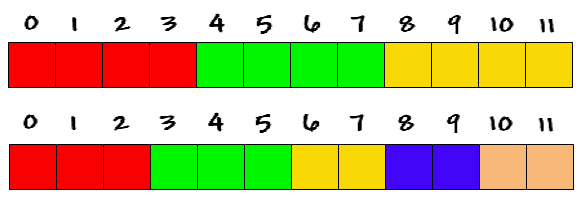
\includegraphics[width=0.6\linewidth]{array_procs_both}
  \caption{12 bodies and 3 computational nodes, 12 bodies and 5 computational nodes}
  \label{fig:3nodes}
\end{figure}
\FloatBarrier

\subsection{The Work repartition}
\label{sec:work_rep}

\subsubsection{Naive repartition}
\label{sec:naive_rep}

This is the most critical part of the implementation, from this depends the efficiency of the whole algorithm. 
Using a naive approach for every step we could simply use the MPI\_Allgatherv operation, to send to all other nodes our updated chunk of bodies and receive all the other chunks from other nodes. Than compute the forces that all other bodies exert on the actual chunk and update the actual chunk bodies positions and speeds. 

A problem of this approach is the big amount of data transferred in each iteration (N bodiesType structures) and the fact that we are computing the same forces between some pairs of bodies in more than one machine. In fact, computing the force that the body A exert on the body B, implicitly we are computing also the force that the body B exert on the body A (force of B on A is negative of A on B). Given a situation like the one described on Figure \ref{fig:nodes}, we can see on Tables \ref{table:t1} and \ref{table:t2} the forces computed by the first two nodes.

\begin{figure}[ht]
  \centering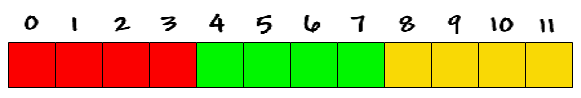
\includegraphics[width=0.6\linewidth]{array_procs_3}
  \caption{12 bodies and 3 computational nodes}
  \label{fig:nodes}
\end{figure}
\FloatBarrier

\begin{table}[]
\centering
\caption{Node 0 - Calculated forces}
\label{table:t1}
\begin{tabular}{l|lllllllllll}
bodies{[}0{]} & 0-1 & 0-2 & 0-3 & \textcolor{red}{0-4} & \textcolor{red}{0-5} & \textcolor{red}{0-6} & \textcolor{red}{0-7}  & 0-8  & 0-9  & 0-10 & 0-11 \\ \hline
bodies{[}1{]} & 1-2 & 1-3 & \textcolor{red}{1-4} & \textcolor{red}{1-5} & \textcolor{red}{1-6} & \textcolor{red}{1-7} & 1-8  & 1-9  & 1-10 & 1-11 &      \\ \hline
bodies{[}2{]} & 2-3 & \textcolor{red}{2-4} & \textcolor{red}{2-5} & \textcolor{red}{2-6} & \textcolor{red}{2-7} & 2-8 & 2-9  & 2-10 & 2-11 &      &      \\ \hline
bodies{[}3{]} & \textcolor{red}{3-4} & \textcolor{red}{3-5} & \textcolor{red}{3-6} & \textcolor{red}{3-7} & 3-8 & 3-9 & 3-10 & 3-11 &      &      &   
\end{tabular}
\end{table}

\begin{table}[]
\centering
\caption{Node 1 - Calculated forces}
\label{table:t2}
\begin{tabular}{l|lllllllllll}
bodies{[}4{]} & \textcolor{red}{4-0} & \textcolor{red}{4-1} & \textcolor{red}{4-2} & \textcolor{red}{4-3} & 4-5 & 4-6 & 4-7  & 4-8  & 4-9  & 4-10 & 4-11 \\ \hline
bodies{[}5{]} & \textcolor{red}{5-0} & \textcolor{red}{5-1} & \textcolor{red}{5-2} & \textcolor{red}{5-3} & 5-6 & 5-7 & 5-8  & 5-9  & 5-10 & 5-11 &      \\ \hline
bodies{[}6{]} & \textcolor{red}{6-0} & \textcolor{red}{6-1} & \textcolor{red}{6-2} & \textcolor{red}{6-3} & 6-7 & 6-8 & 6-9  & 6-10 & 6-11 &      &      \\ \hline
bodies{[}7{]} & \textcolor{red}{7-0} & \textcolor{red}{7-1} & \textcolor{red}{7-2} & \textcolor{red}{7-3} & 7-8 & 7-9 & 7-10 & 7-11 &      &      &     
\end{tabular}
\end{table}

As we can notice from Tables \ref{table:t1} and \ref{table:t2}, forces between the pairs highlighted in red are calculated by both Node 0 and Node 1. For each node we calculate the forces for 38 pairs, that means 114 pairs (38 x 3) in total. The number of possible pairs is 66, so we are doing about 1.7 times the needed work. \\
An approximation of the computation is shown on the Equation \ref{eq:eq1}). The first O represents the computation of the forces between the chunk's bodies and all the other bodies, while the second O represents the computation of the forces between the chunk's bodies. \\

\begin{equation} 
\label{eq:eq1}
\begin{split}
Computation & = O(\lceil\frac{N}{P}\rceil * \lceil\frac{N}{P}\rceil * (P-1)) +  O(\sum_{i=1}^{\lceil\frac{N}{P}\rceil} {(\lceil\frac{N}{P}\rceil-i)})\\
 & = O(\lceil\frac{N^2}{P}\rceil)
\end{split}
\end{equation}

With this approach for each iteration we send O(N/P) bodies and we receive O(N-N/P) bodies, that means an O(N) communication. For the computation we have the O(N\textsuperscript{2}/P) for the force computation, and an O(N/P)for the velocities and the positions computation.

\subsubsection{Optimized repartition}
\label{sec:opt_rep}
The aim of a good repartition is to not repeat the same work on different nodes. Following this objective the idea is, given a pair of chunks, half of the forces that two bodies from different chunks exert on each other are calculated by one node, and half by the other. The ripartition is clarify on the Figures \ref{fig:pr1}, \ref{fig:pr2} and \ref{fig:pr3}.


\begin{figure}[ht]
\centering
\begin{subfigure}{.35\textwidth}
  \centering
  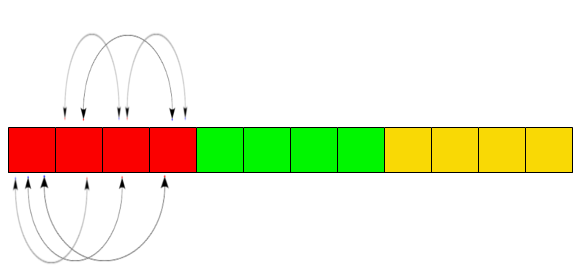
\includegraphics[width=1\linewidth]{array_proc_0_b_0}
\end{subfigure}%
\begin{subfigure}{.35\textwidth}
  \centering
  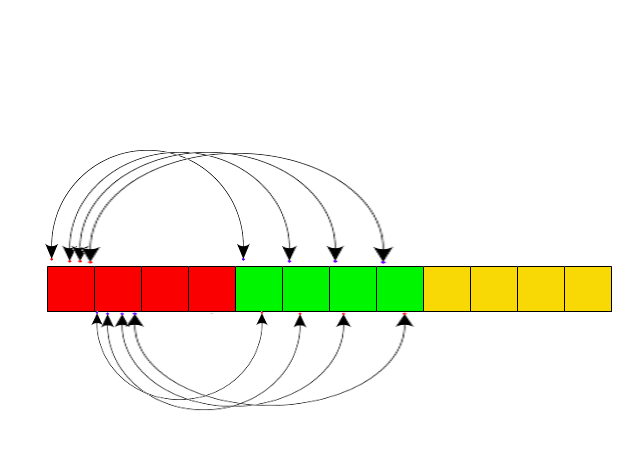
\includegraphics[width=1\linewidth]{array_proc_0_b_1}
\end{subfigure}\\ %
\begin{subfigure}{.35\textwidth}
  \centering
  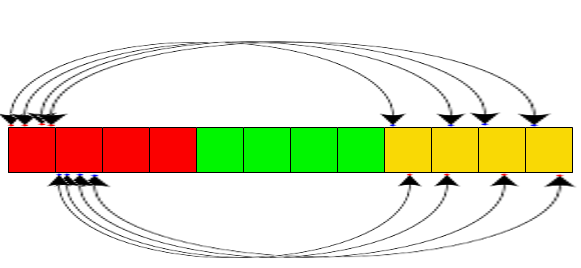
\includegraphics[width=1\linewidth]{array_proc_0_b_2}
\end{subfigure}
  \caption{Forces computed by Node 0 (6+8+8=22)}
  \label{fig:pr1}
\end{figure}
\FloatBarrier


\begin{figure}[ht]
\centering
\begin{subfigure}{.35\textwidth}
  \centering
  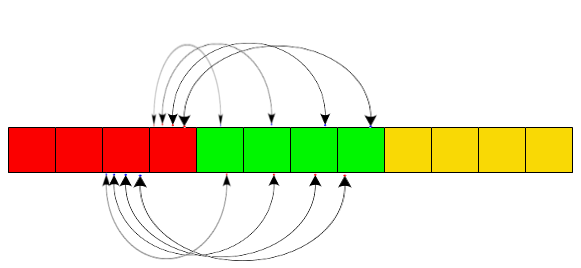
\includegraphics[width=1\linewidth]{array_proc_1_b_0}
\end{subfigure}%
\begin{subfigure}{.35\textwidth}
  \centering
  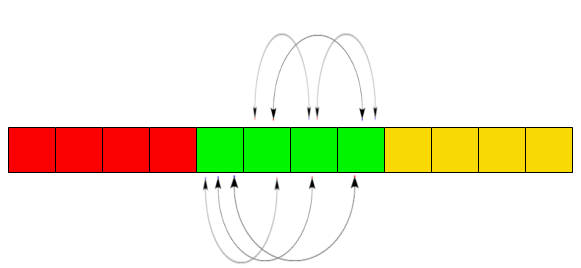
\includegraphics[width=1\linewidth]{array_proc_1_b_1}
\end{subfigure}\\ %
\begin{subfigure}{.35\textwidth}
  \centering
  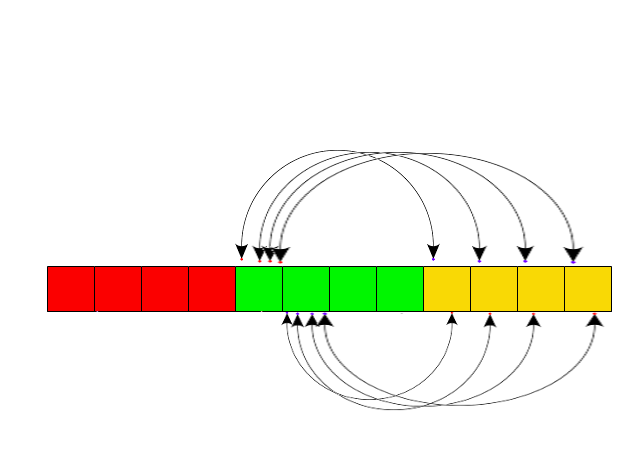
\includegraphics[width=1\linewidth]{array_proc_1_b_2}
\end{subfigure}
  \caption{Forces computed by Node 1 (8+6+8=22)}
  \label{fig:pr2}
\end{figure}
\FloatBarrier


\begin{figure}[ht]
\centering
\begin{subfigure}{.35\textwidth}
  \centering
  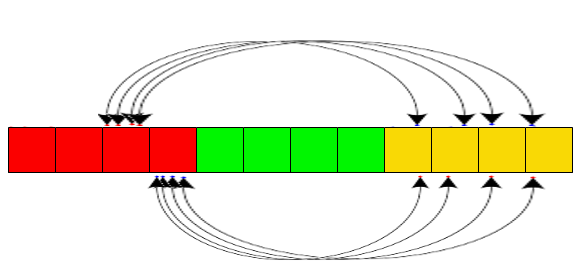
\includegraphics[width=1\linewidth]{array_proc_2_b_0}
\end{subfigure}%
\begin{subfigure}{.35\textwidth}
  \centering
  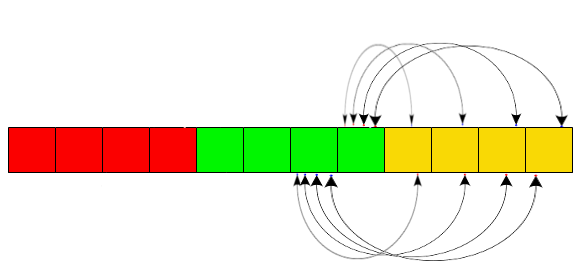
\includegraphics[width=1\linewidth]{array_proc_2_b_1}
\end{subfigure}\\ %
\begin{subfigure}{.35\textwidth}
  \centering
  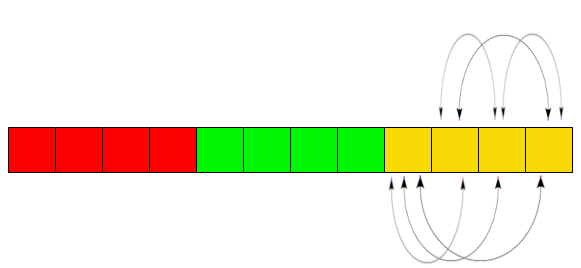
\includegraphics[width=1\linewidth]{array_proc_2_b_2}
\end{subfigure}
  \caption{Forces computed by Node 2 (8+8+6=22)}
  \label{fig:pr3}
\end{figure}
\FloatBarrier

Proceeding in this way, the forces between all pairs of bodies are calculated only one time per step. Each node computes the forces of 22 pairs. We have 3 nodes, so 3 times 22 is 66 that correspond to the number of possible pairs. No useful work is done. The approximated computational time is shown in the Equation \ref{eq:eq2}. The first O represents the computation of the forces between the chunk's bodies and the bodeis of other chunks, while the second O represents the computation of the forces between the chunk's bodies.

\begin{equation} \label{eq:eq2}
\begin{split}
Complexity & = O(\lceil\frac{N}{P}\rceil * (\lceil\frac{N}{P}\rceil * \frac{1}{2}) * (P-1)) +  O(\sum_{i=1}^{\lceil\frac{N}{P}\rceil} {(\lceil\frac{N}{P}\rceil-i)})\\
 & = O(\lceil\frac{N^2}{2P}\rceil)
\end{split}
\end{equation}

\subsection{The final solution}
\label{sec:comm_comp}

\subsubsection{Communication VS Computation}
\label{sec:comm_comp}
The communication is a common bottleneck on lots of parallel implementations. The data exchange between nodes should be reduced at the minimum in order to obtain good performances. The problem with the N body algorithm is that at every step we need the updated information (positions, velocities) of all other bodies of the system in order to correctly compute the forces of the assigned chunk. That means an exchange of data for every step. To gain performances we have to find a good compromise between the data exchange and the work to do on each node. In particular, we have to maximize the ratio \textit{computation/communication}. Due to the fact that the force computation is the most expensive part of the algorithm and that we want to exchange as less data as possible, a good compromise is the following. At the beginning, we broadcast to all the nodes the bodies (MPI\_Bcast). Than for each step, each node calculates the forces for the assigned pairs (the one described on Section \ref{sec:opt_rep}), after that uses an MPI\_Allreduce operation to sum all the calculated forces by all the nodes and as the last thing it computes the velocities and positions for all the bodies. Proceeding i this way, we exchange only an array of N elements containing the forces calculated for the assigned pairs. The major problem with this approach, is that we calculate the positions and velocities of all the bodies in every node, that represent a duplication of work. An alternative could be to calculate in each node only the velocities and the positions of the bodies of the assigned chunk, but doing this we have to share with the other nodes also this information. The decision so, is between computing the N velocities and positions in all the nodes or exchange more data with the other nodes. In the following two sections the two approaches are shown is details, using some images to clarify the idea behind each of them.

\subsubsection{Approach one}
\label{sec:app_1}

With this approach we want to reduce the communication between the nodes. 
Phase A (Figure \ref{fig:A2}) is executed at the begin. Phases B, C, D (Figures \ref{fig:B2}, \ref{fig:C2}, \ref{fig:D2}) are executed inside a loop (for each step). An approximation of the whole complexity and of the total amount of data exchanged per step is presented in Equations \ref{eq:comp_app1} and \ref{eq:com_app1}.

\begin{figure}[ht]
  \centering
  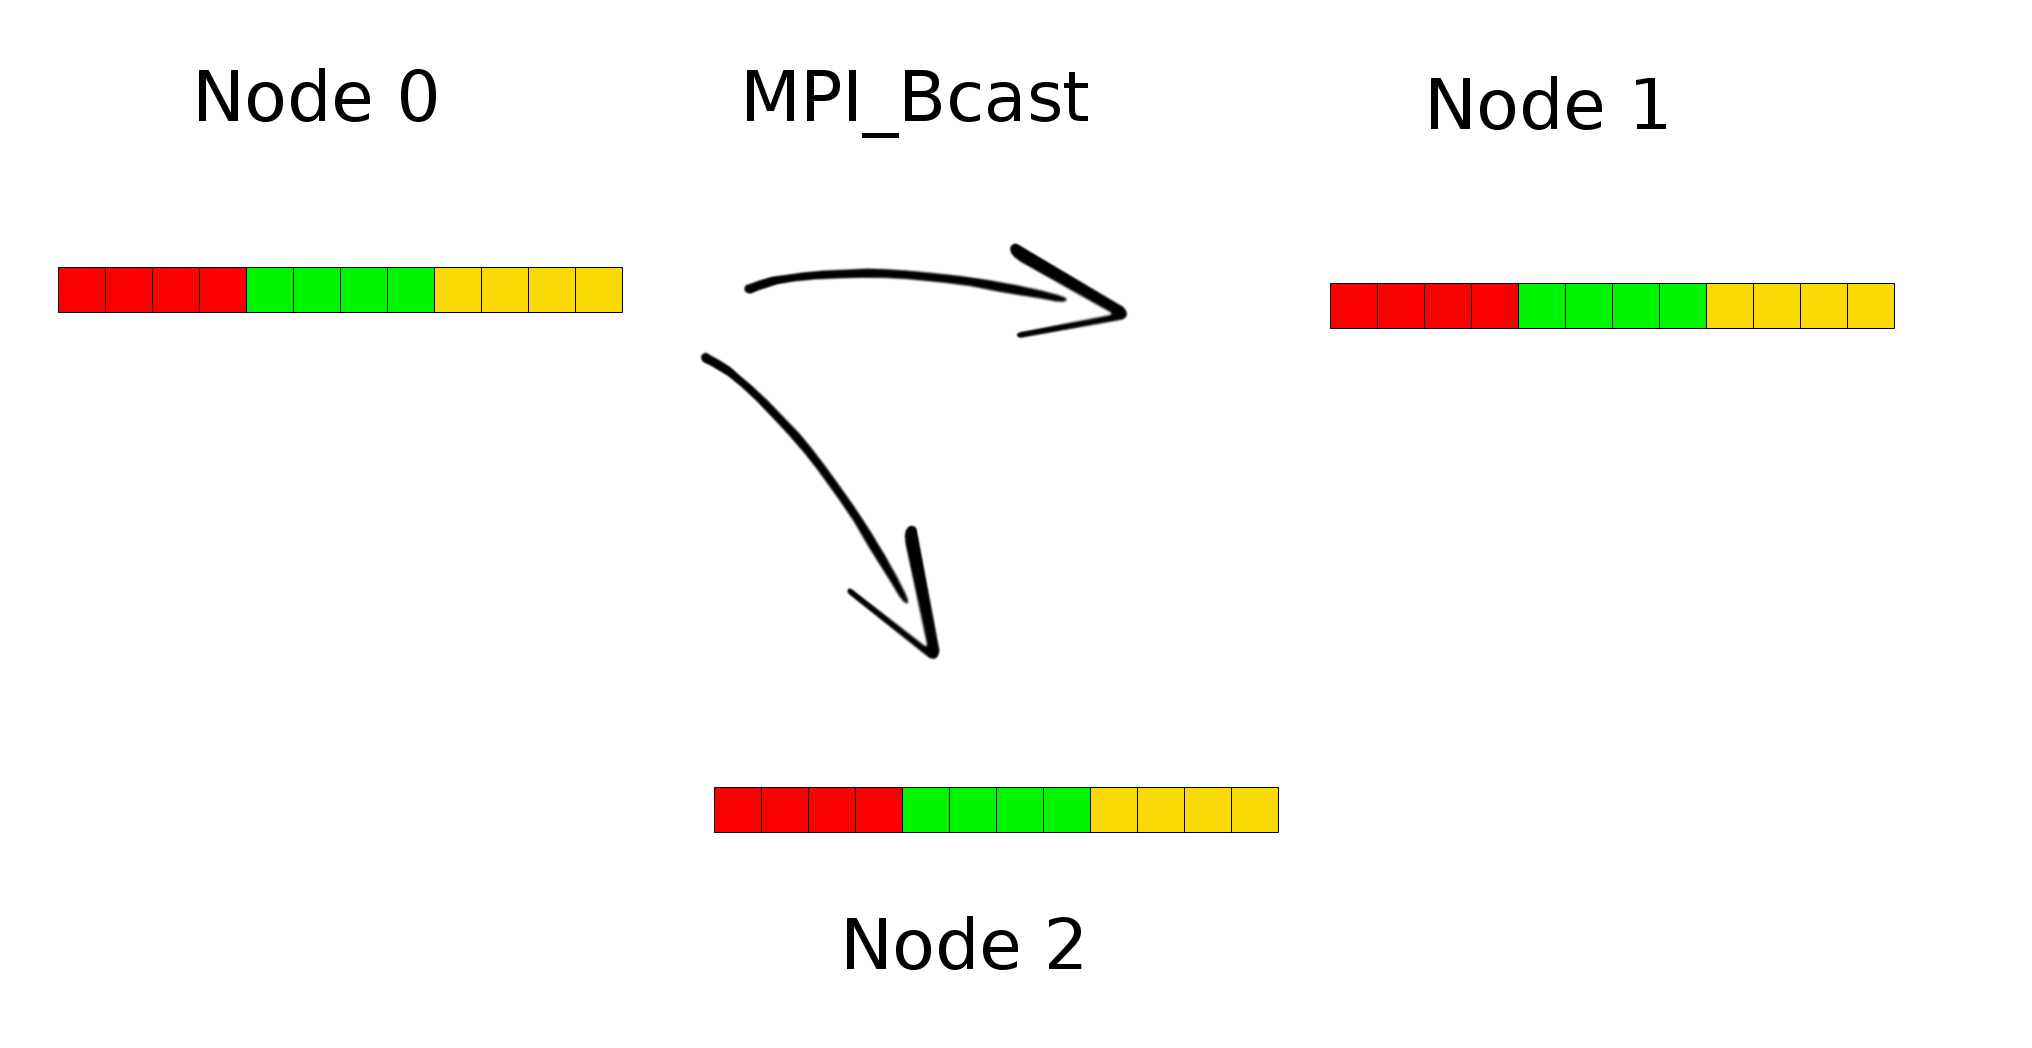
\includegraphics[width=0.5\linewidth]{broadcast}
  \caption{A - Broadcast the bodies to all the nodes}
  \label{fig:A2}
\end{figure}
\FloatBarrier

\begin{figure}[ht]
\begin{subfigure}{.5\textwidth}
  \centering
  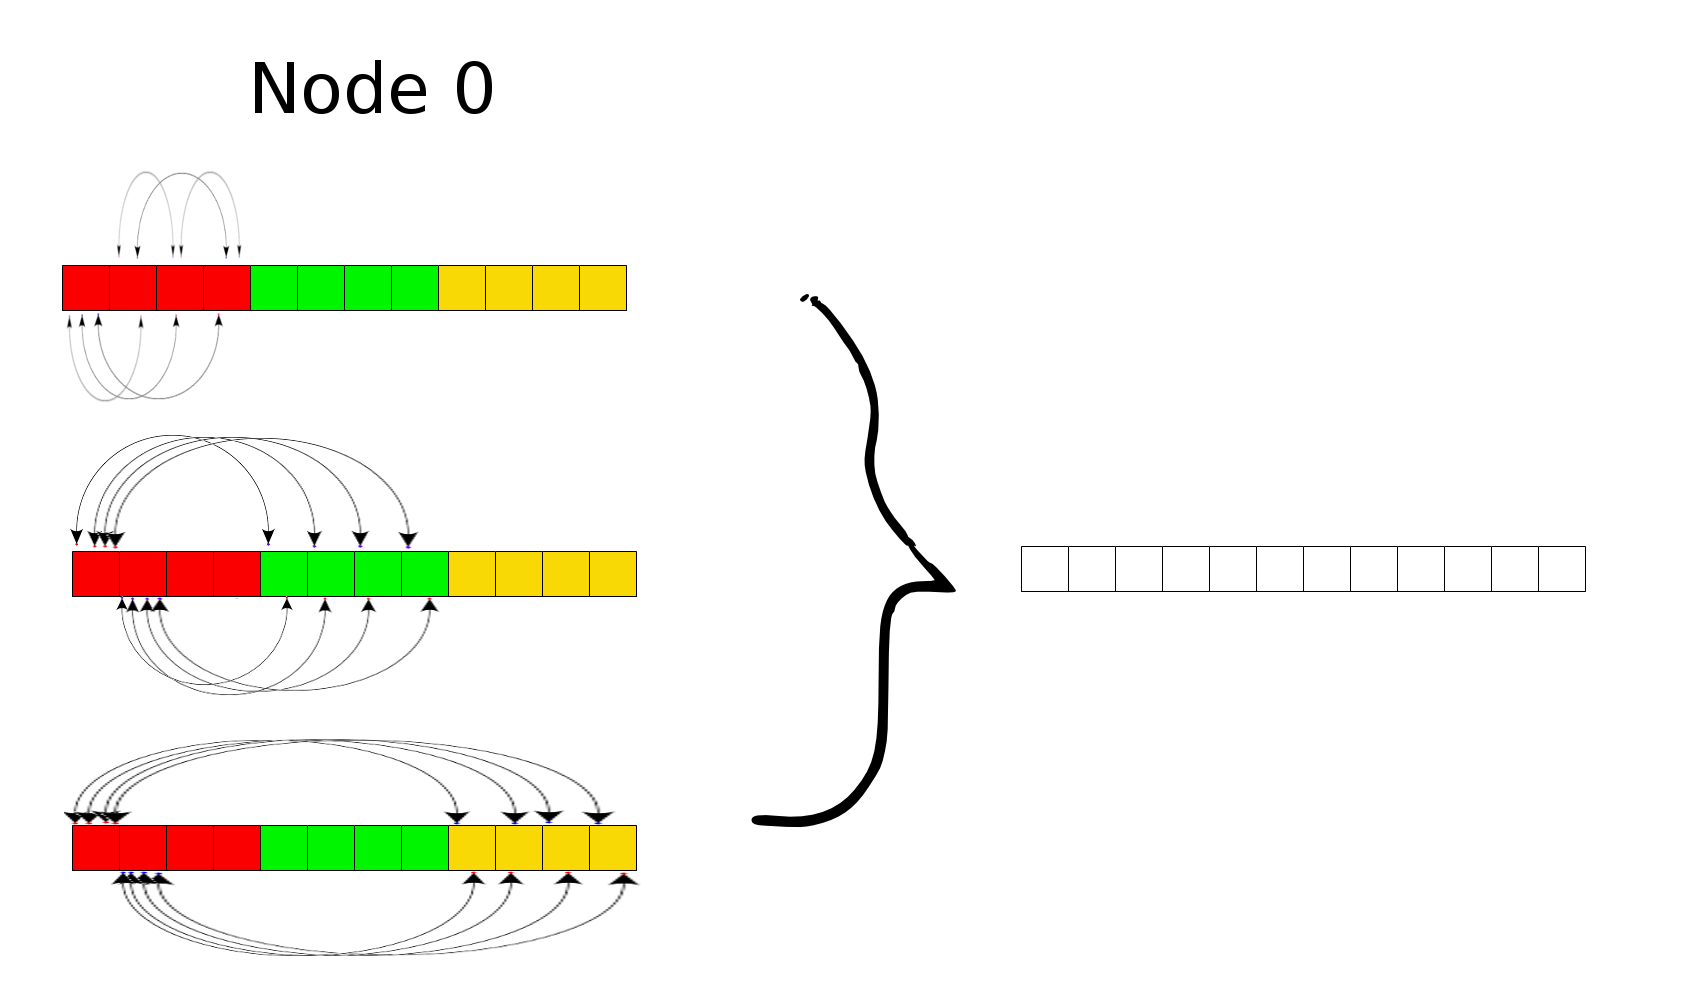
\includegraphics[width=1\linewidth]{force_calculation_0}
\end{subfigure} %
\begin{subfigure}{.5\textwidth}
  \centering
  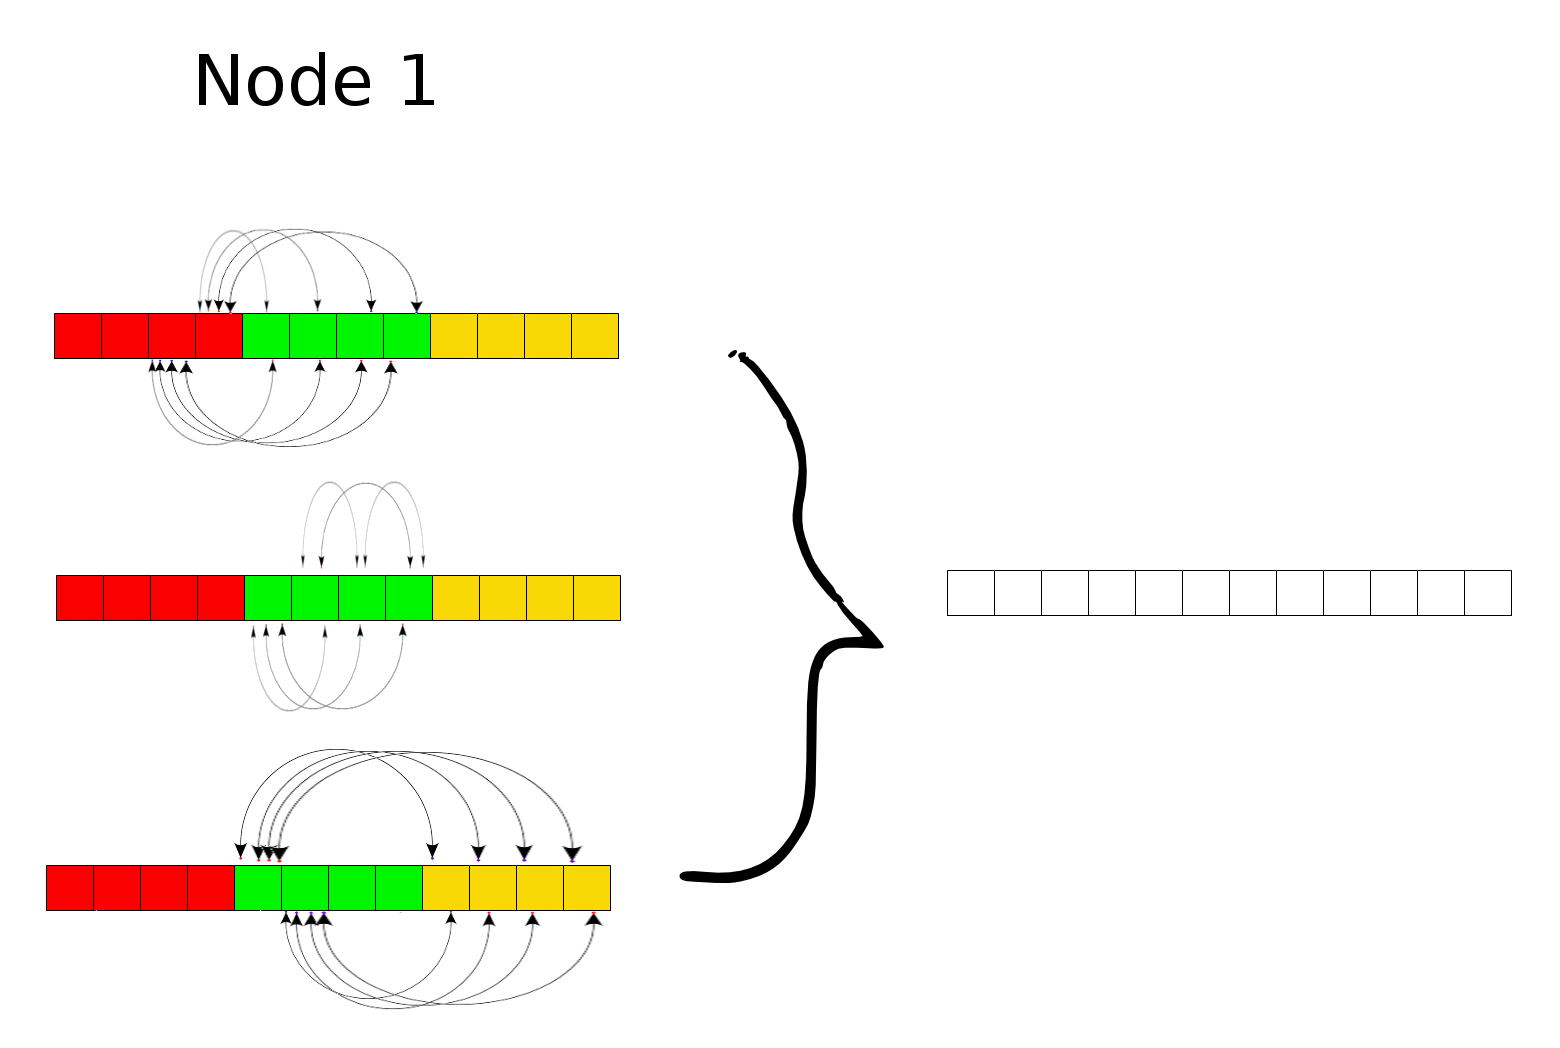
\includegraphics[width=1\linewidth]{force_calculation_1}
\end{subfigure} \\ %
\begin{subfigure}{\textwidth}
  \centering
  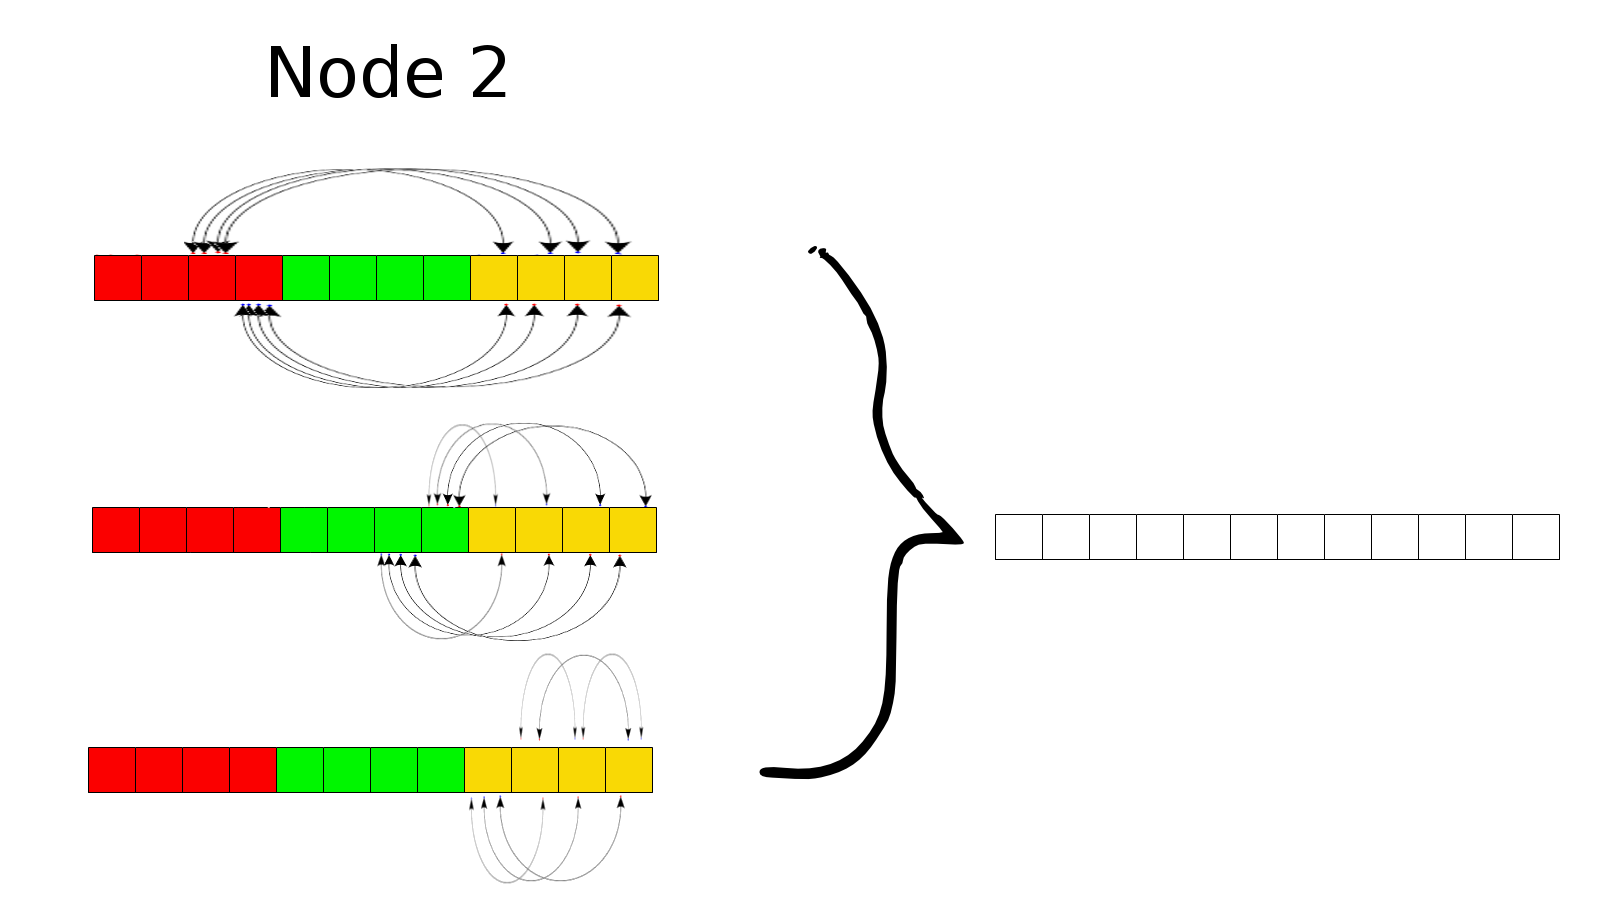
\includegraphics[width=0.5\linewidth]{force_calculation_2}
\end{subfigure}
  \caption{B - Forces computation, the results are put in a vector}
  \label{fig:B2}
\end{figure}
\FloatBarrier

\begin{figure}
\centering
\begin{minipage}{.45\textwidth}
  \centering
  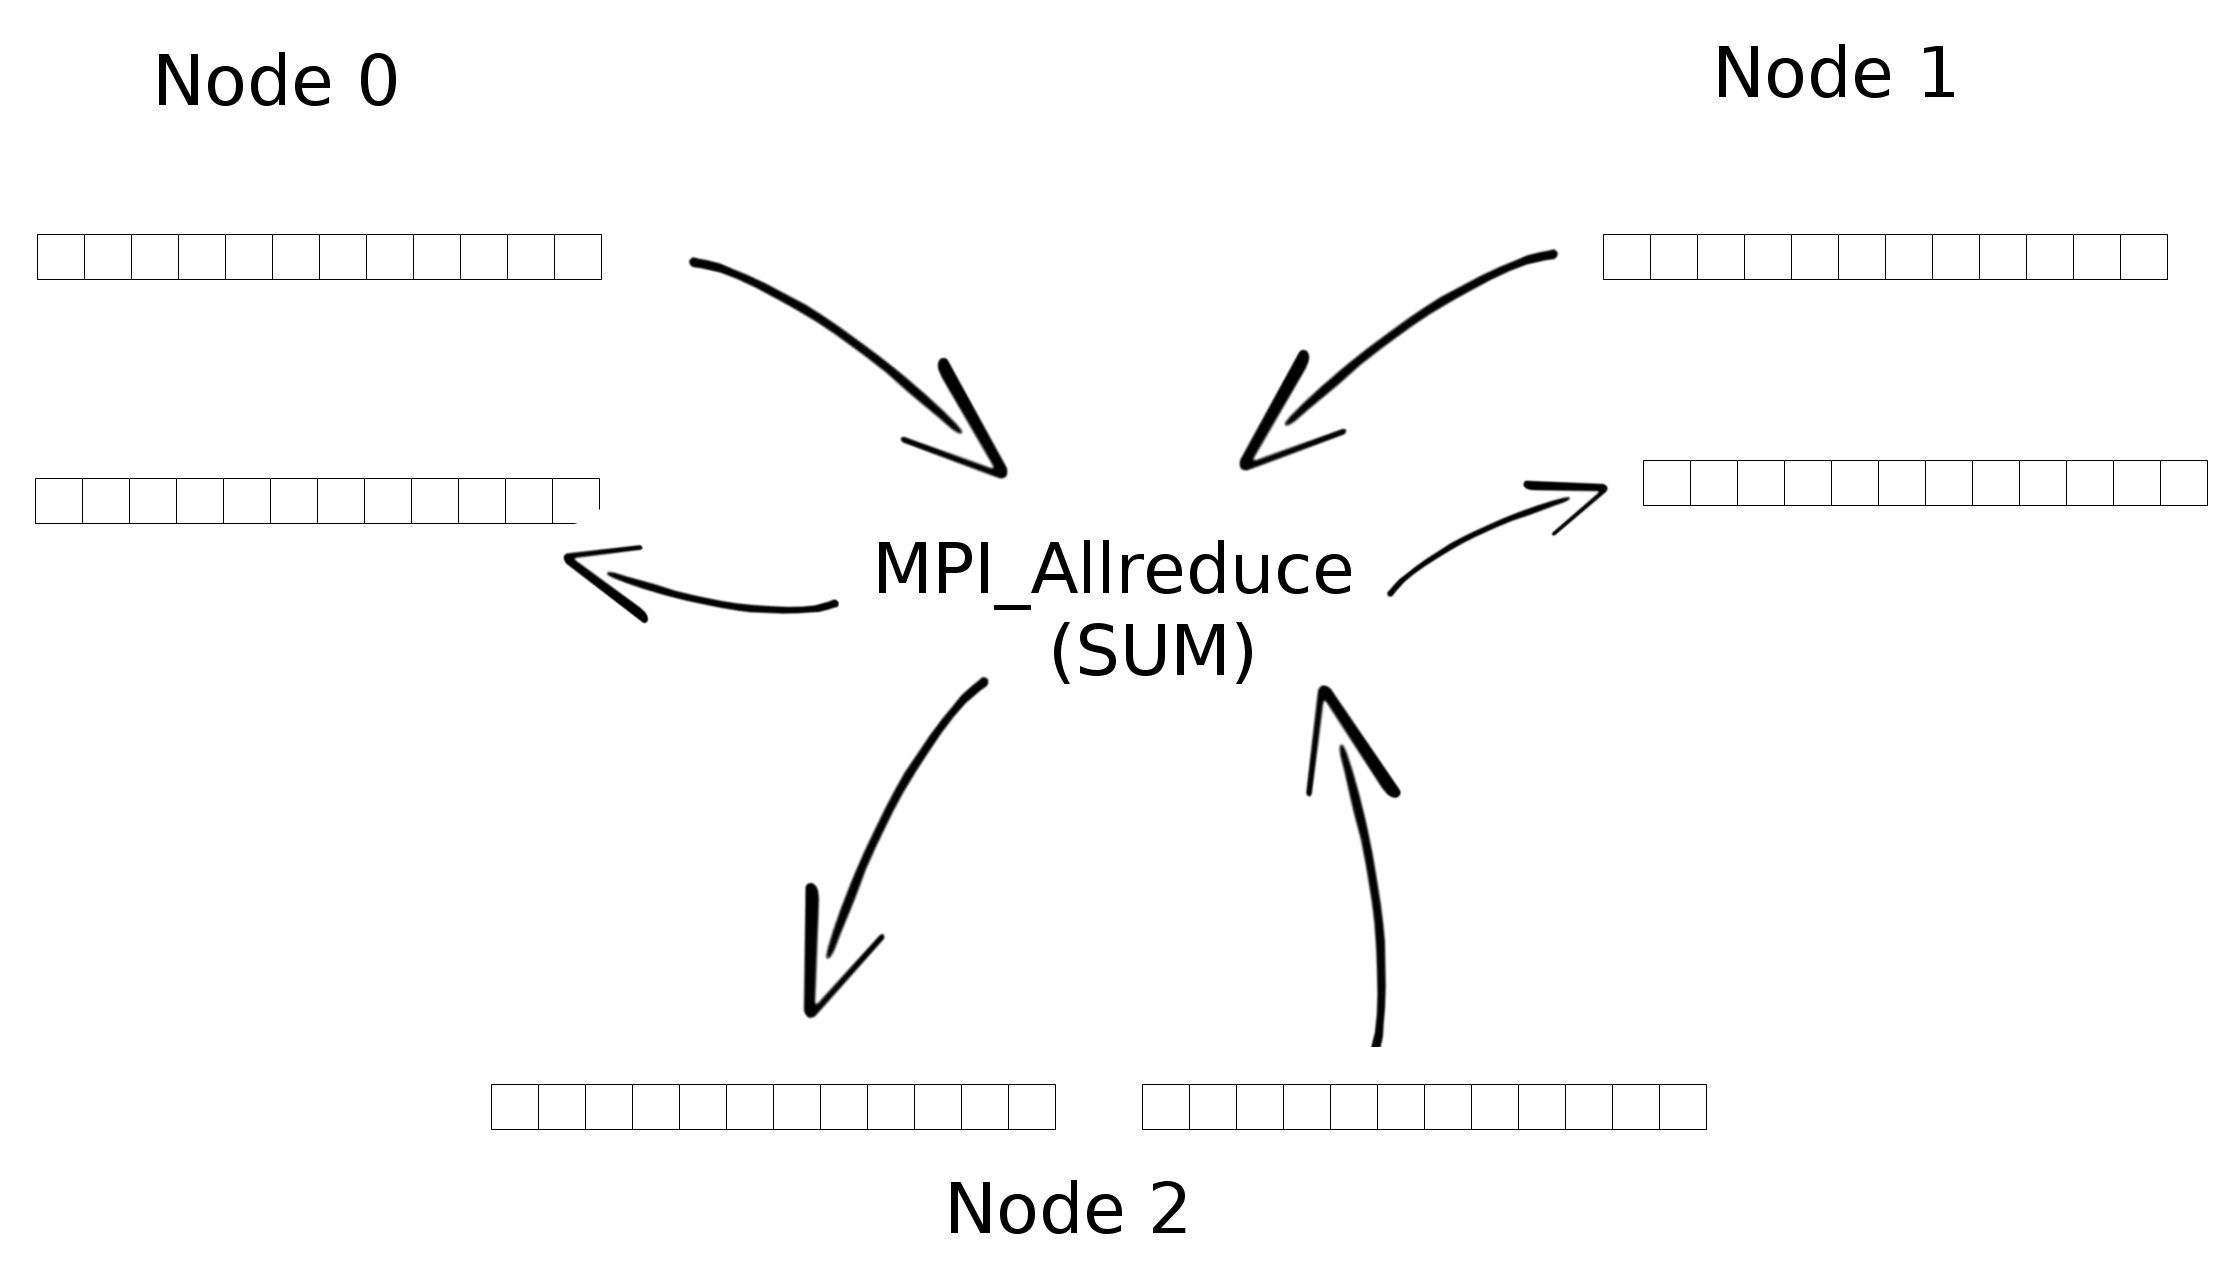
\includegraphics[width=1\linewidth]{MPI_all_reduce}
  \captionof{figure}{C- Forces reduction, sum all the vectors of forces calculated by different nodes}
  \label{fig:C2}
\end{minipage}%
\begin{minipage}{.45\textwidth}
  \centering
  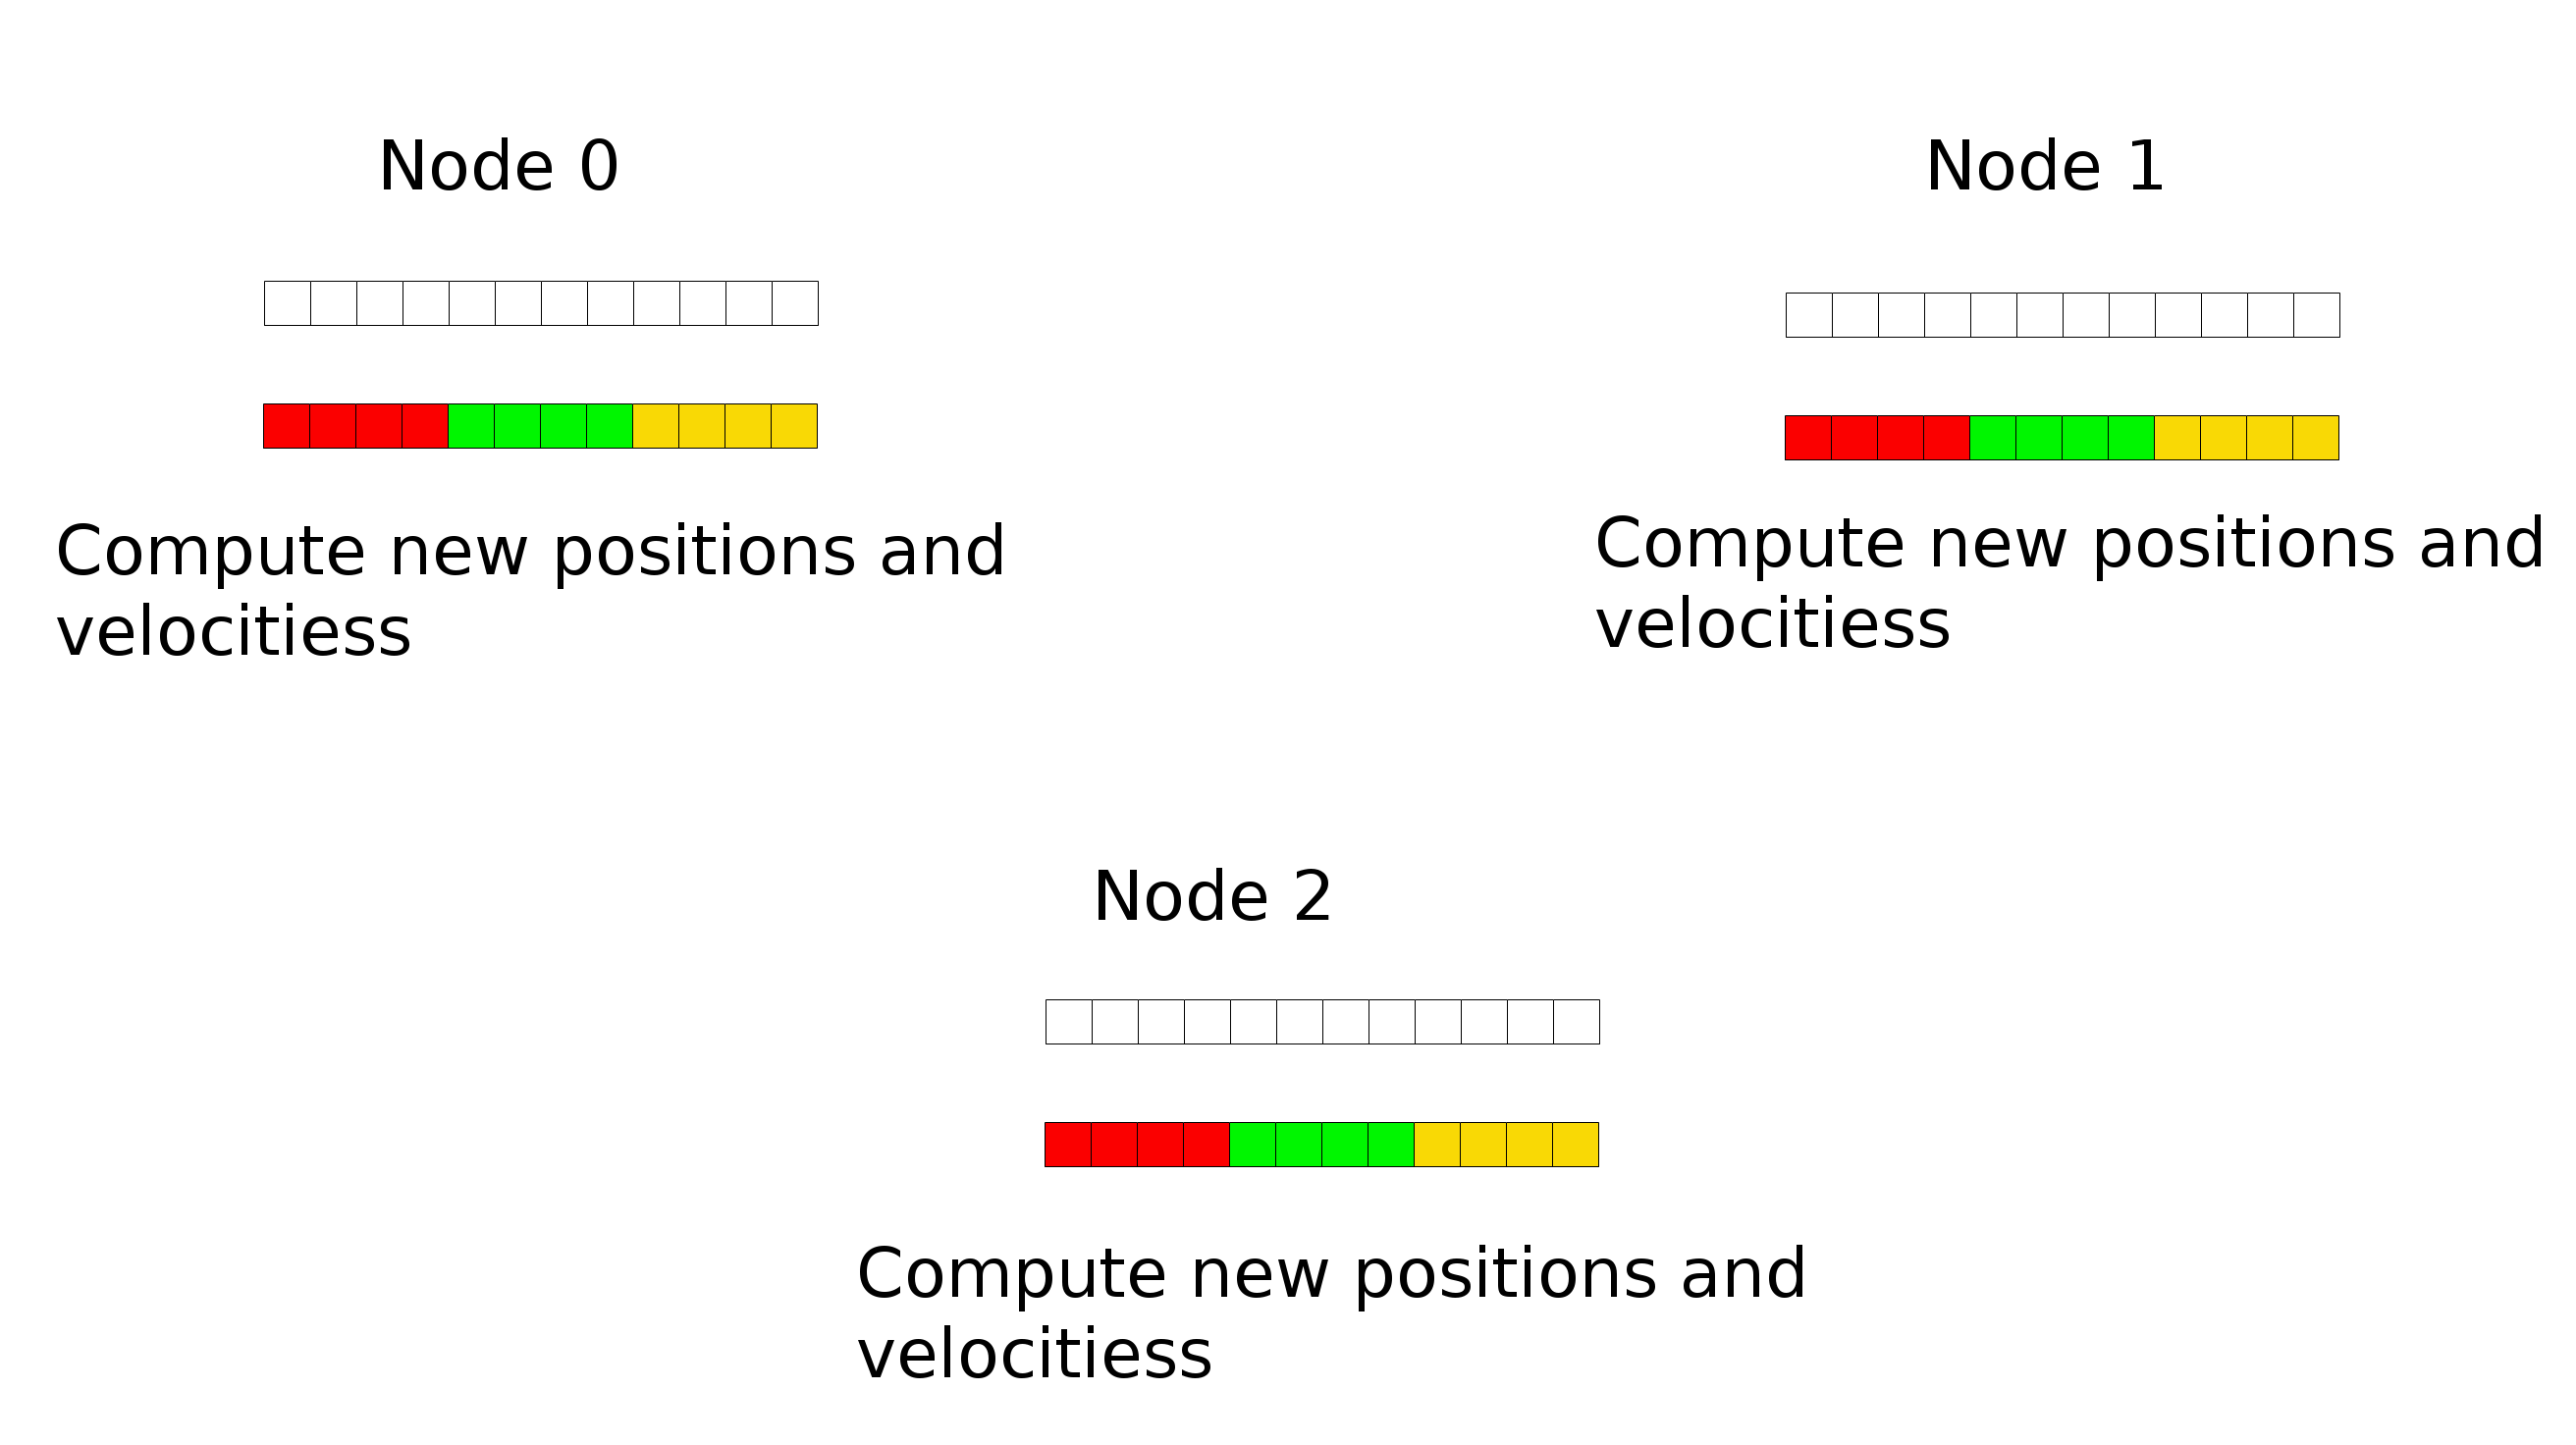
\includegraphics[width=1\linewidth]{compute_positions}
  \captionof{figure}{D - Update positions and velocities for all the bodies}
  \label{fig:D2}
\end{minipage}
\end{figure}
\FloatBarrier

\begin{equation} \label{eq:comp_app1}
\begin{split}
Complexity (per step) & = O(\lceil\frac{N^2}{2P}\rceil)) + O(N) + O(N)\\
 & = O(\lceil\frac{N^2}{2P}\rceil)
\end{split}
\end{equation}

\begin{equation} \label{eq:com_app1}
\begin{split}
Communication (per step) & = O(N)*sizeof(double)
\end{split}
\end{equation}

\subsubsection{Approach two}
\label{sec:app_1}
Phase A (Figure \ref{fig:A1}) is executed at the begin. Phases B, C, D, E (Figures \ref{fig:B1}, \ref{fig:C1}, \ref{fig:D1}, \ref{fig:E1}) are executed inside a loop (for each step). An approximation of the whole complexity and of the total amount of data exchanged per step is presented in Equations \ref{eq:comp_app2} and \ref{eq:com_app2}.

\begin{figure}[ht]
  \centering
  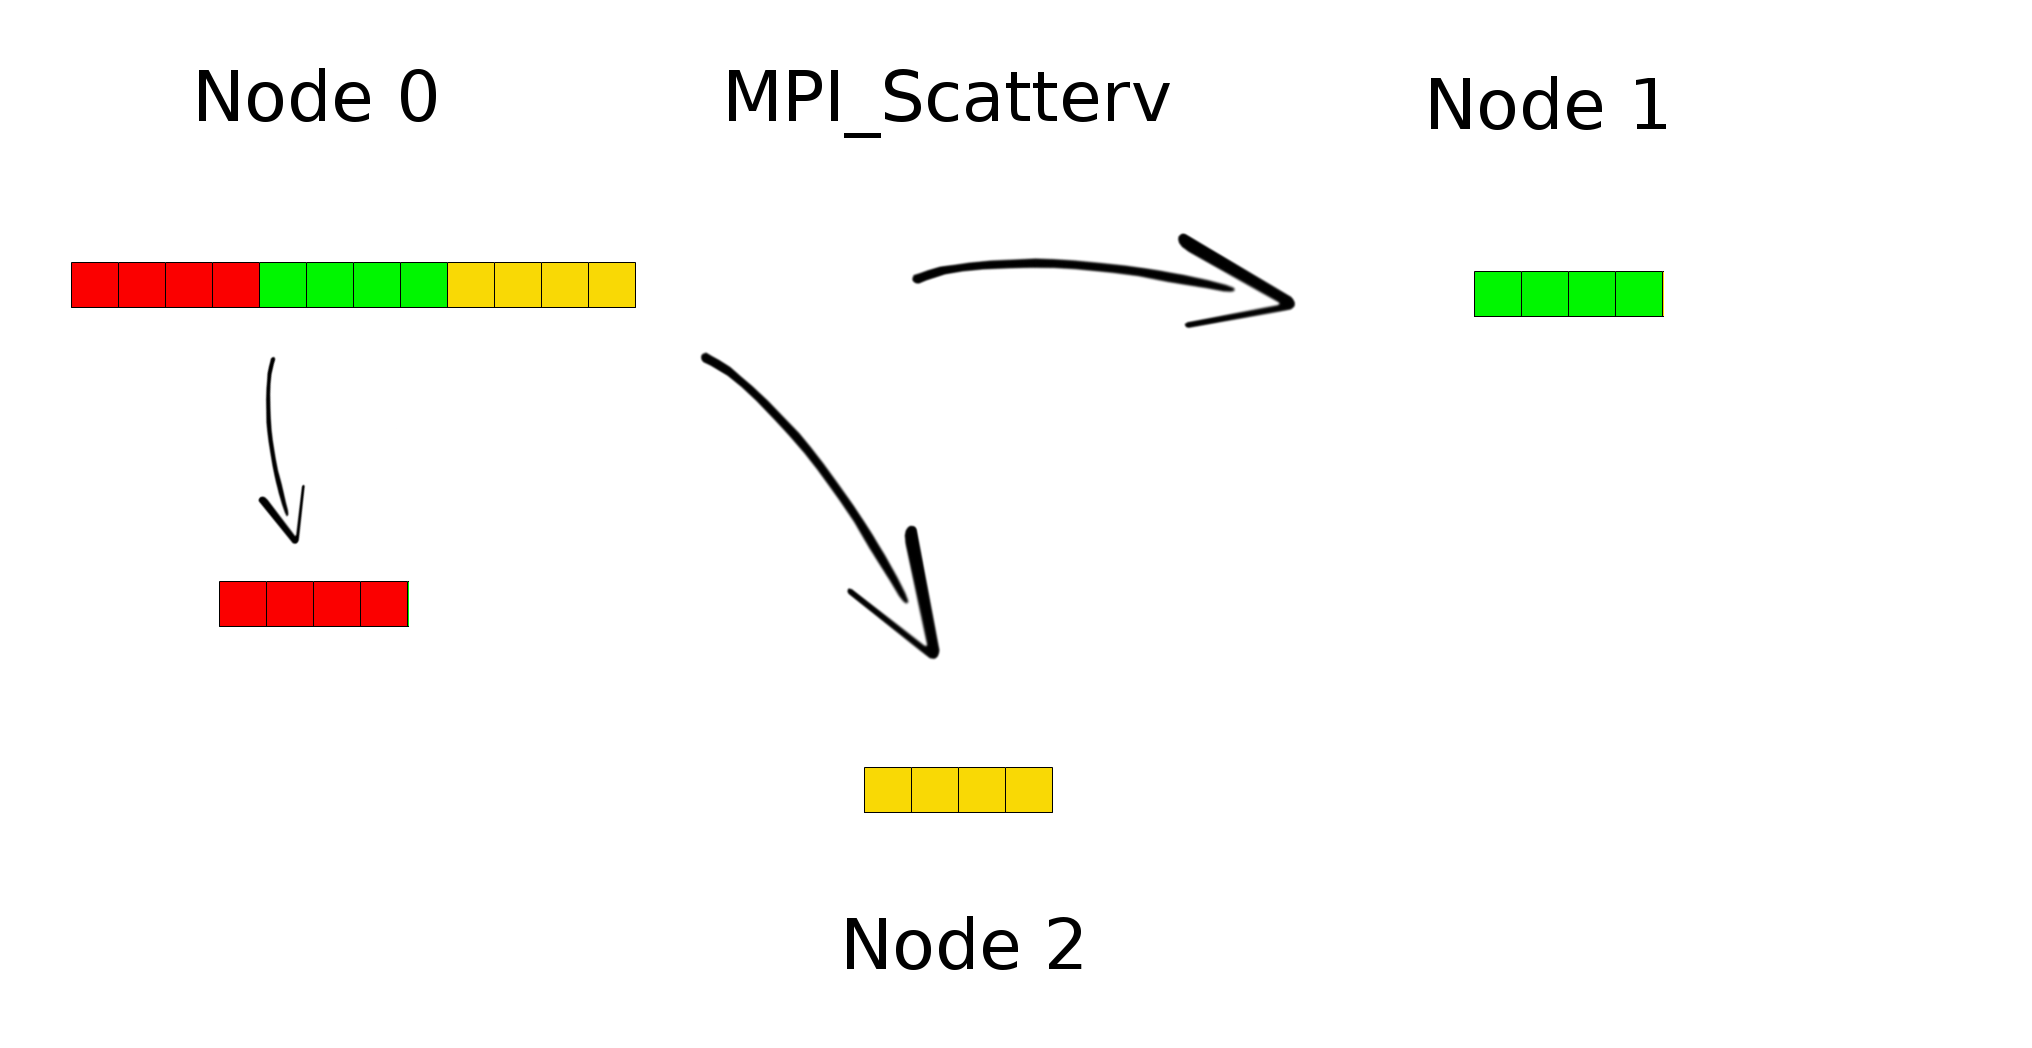
\includegraphics[width=0.6\linewidth]{scatter}
  \caption{A - Scatter the bodies to the nodes}
  \label{fig:A1}
\end{figure}
\FloatBarrier

\begin{figure}[ht]
  \centering
  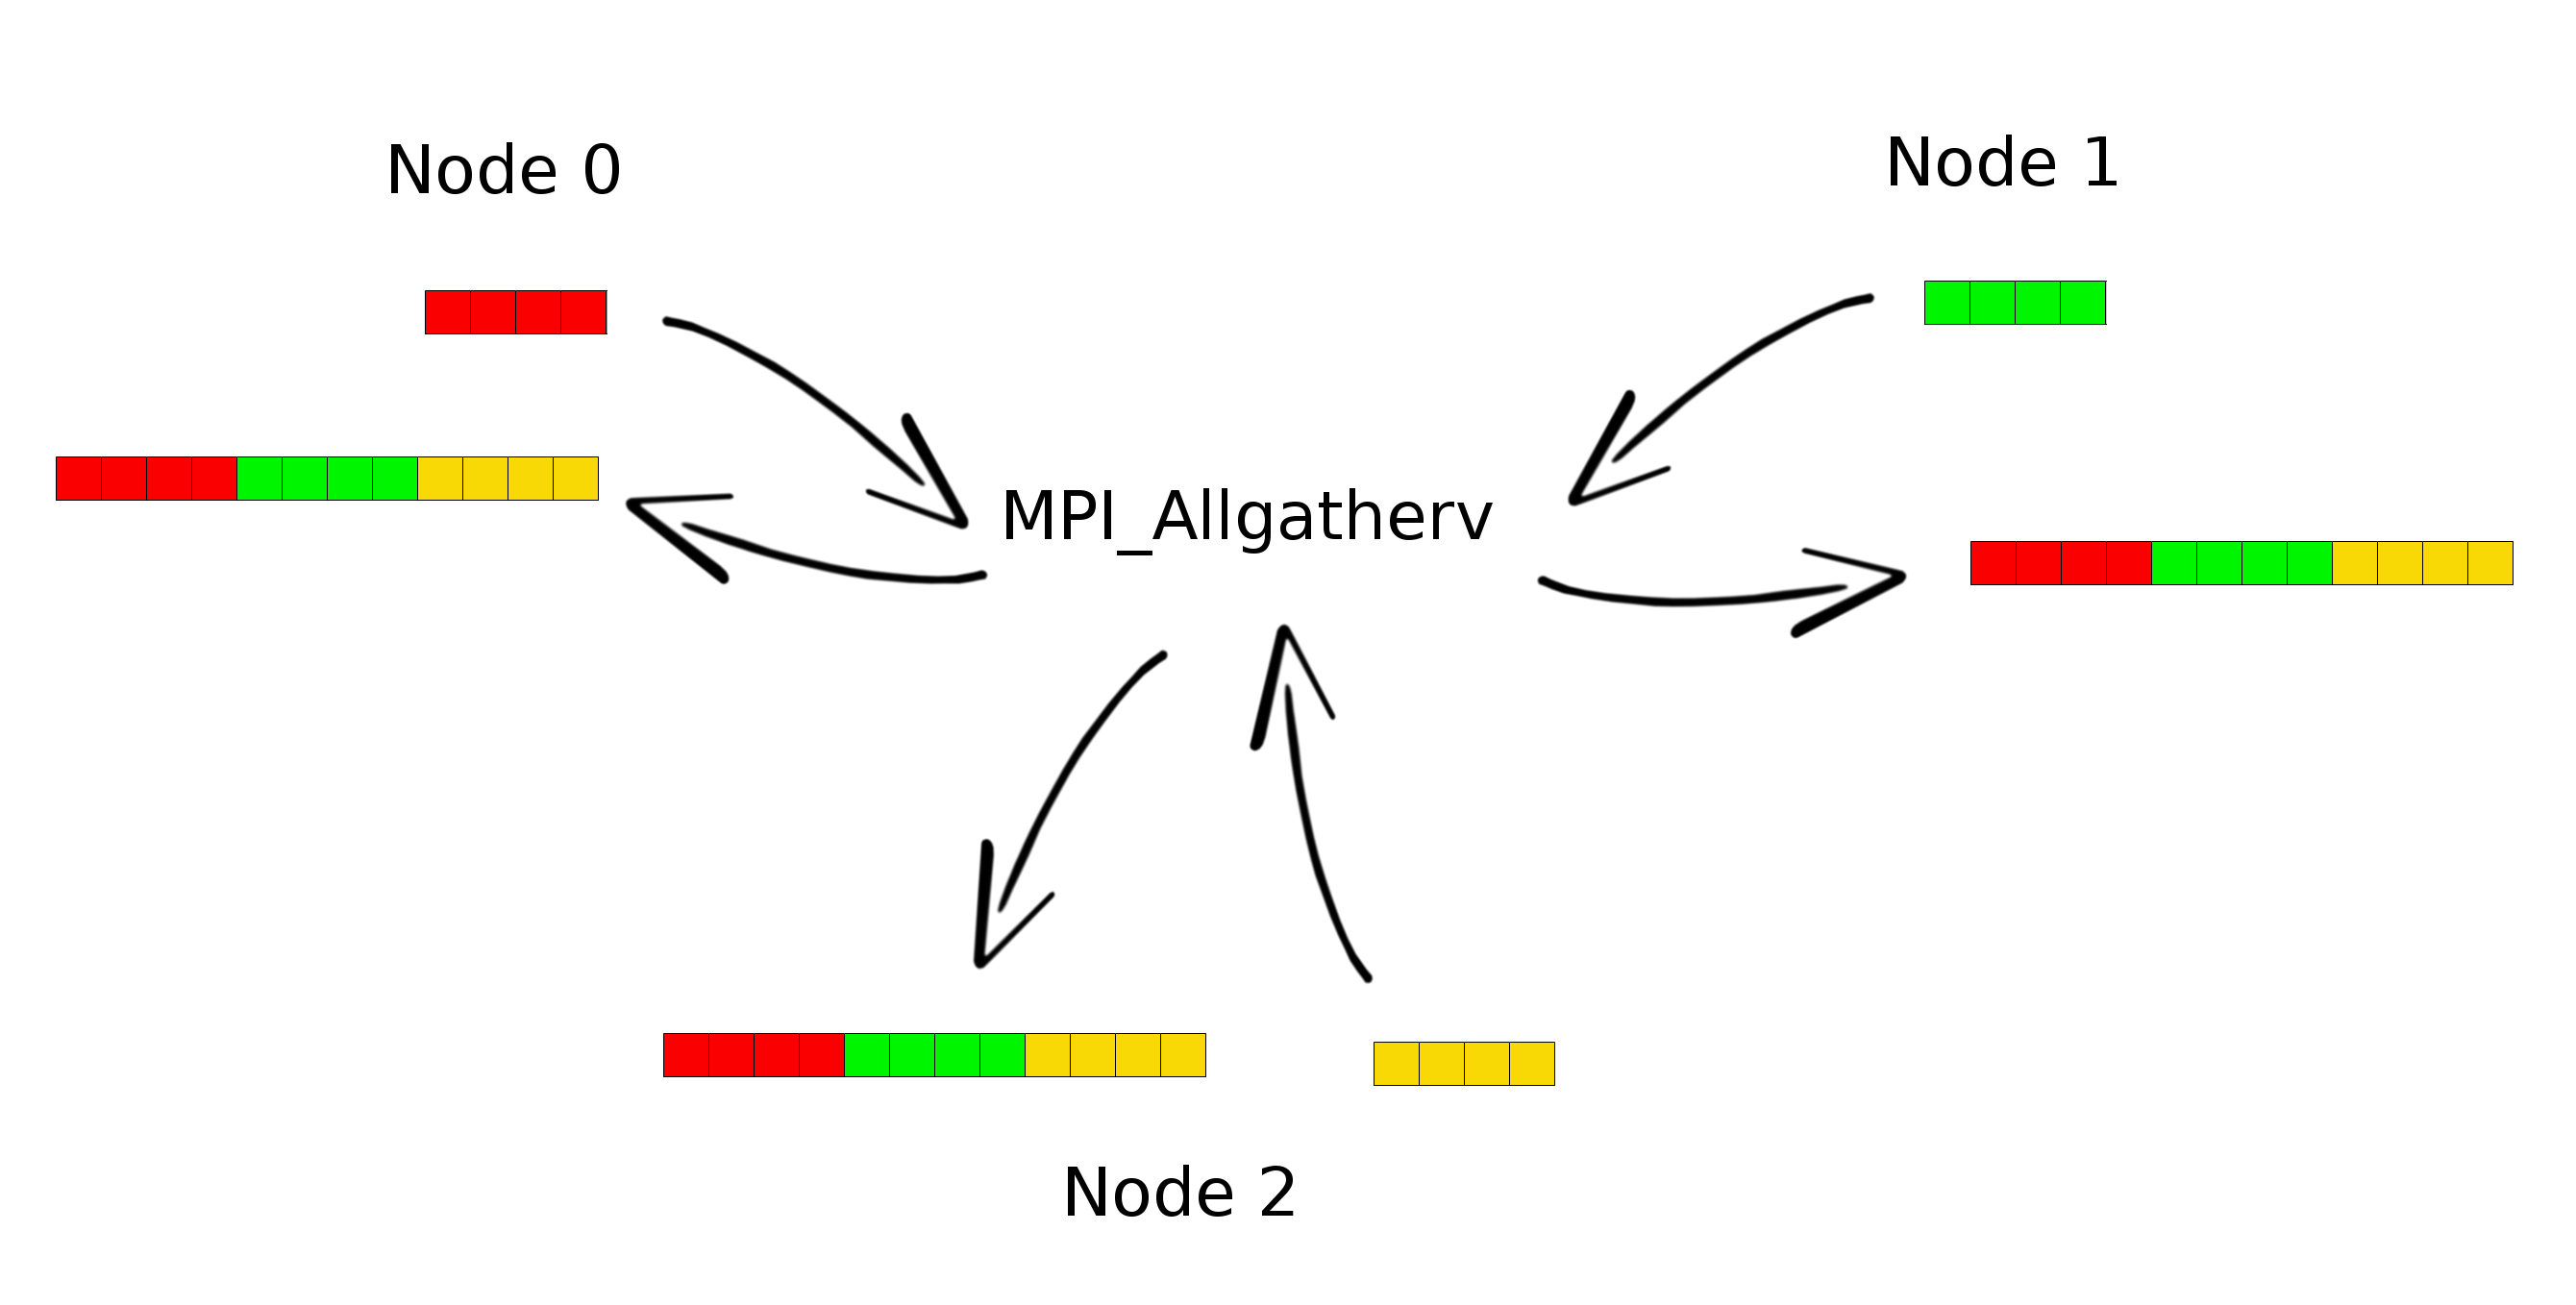
\includegraphics[width=0.5\linewidth]{MPI_all_gather}
  \caption{B - Collect updated bodies from other nodes}
  \label{fig:B1}
\end{figure}
\FloatBarrier

\begin{figure}[ht]
\begin{subfigure}{.5\textwidth}
  \centering
  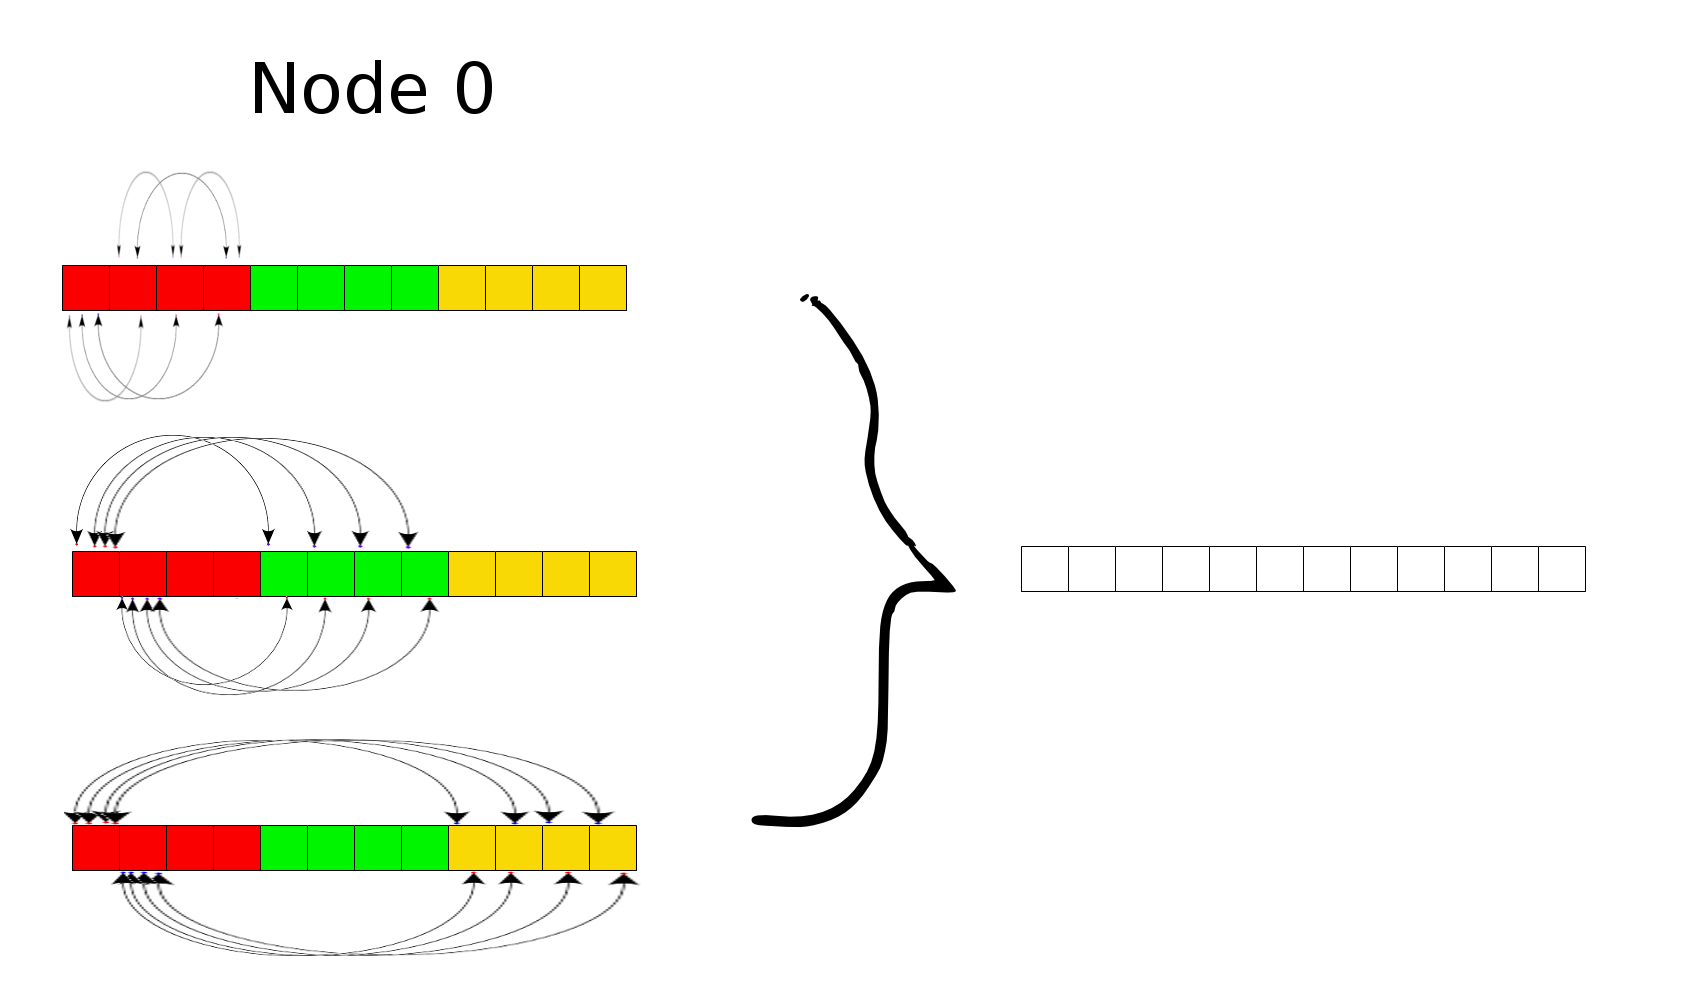
\includegraphics[width=1\linewidth]{force_calculation_0}
\end{subfigure} %
\begin{subfigure}{.5\textwidth}
  \centering
  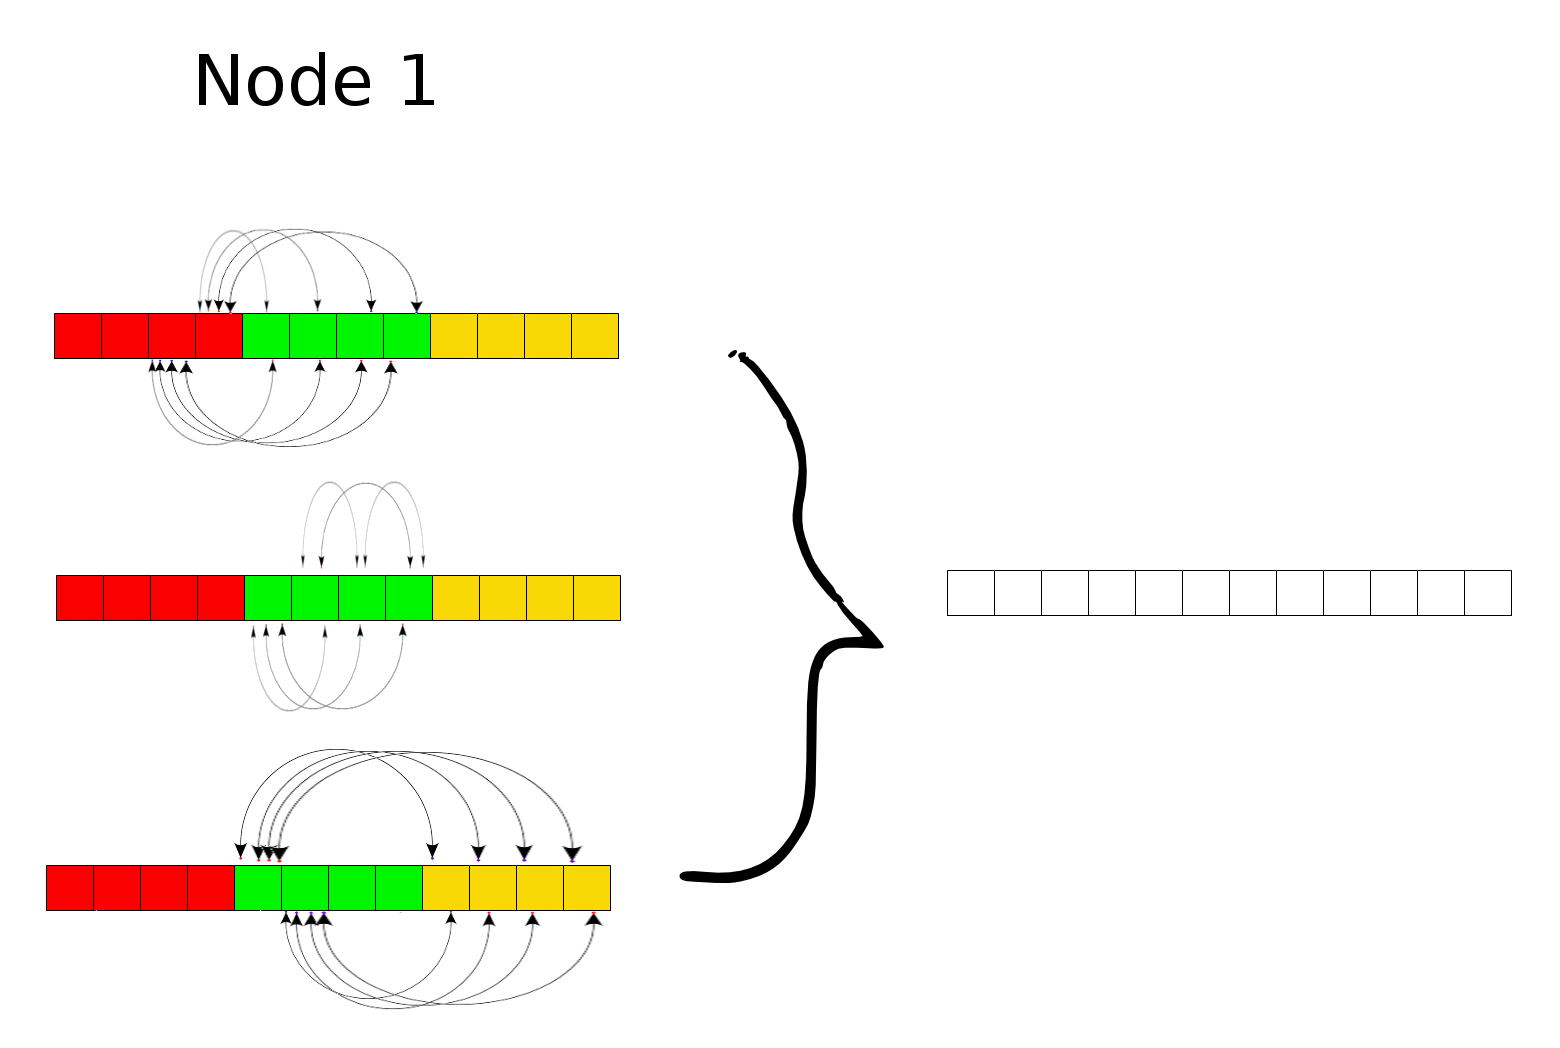
\includegraphics[width=1\linewidth]{force_calculation_1}
\end{subfigure} \\ %
\begin{subfigure}{\textwidth}
  \centering
  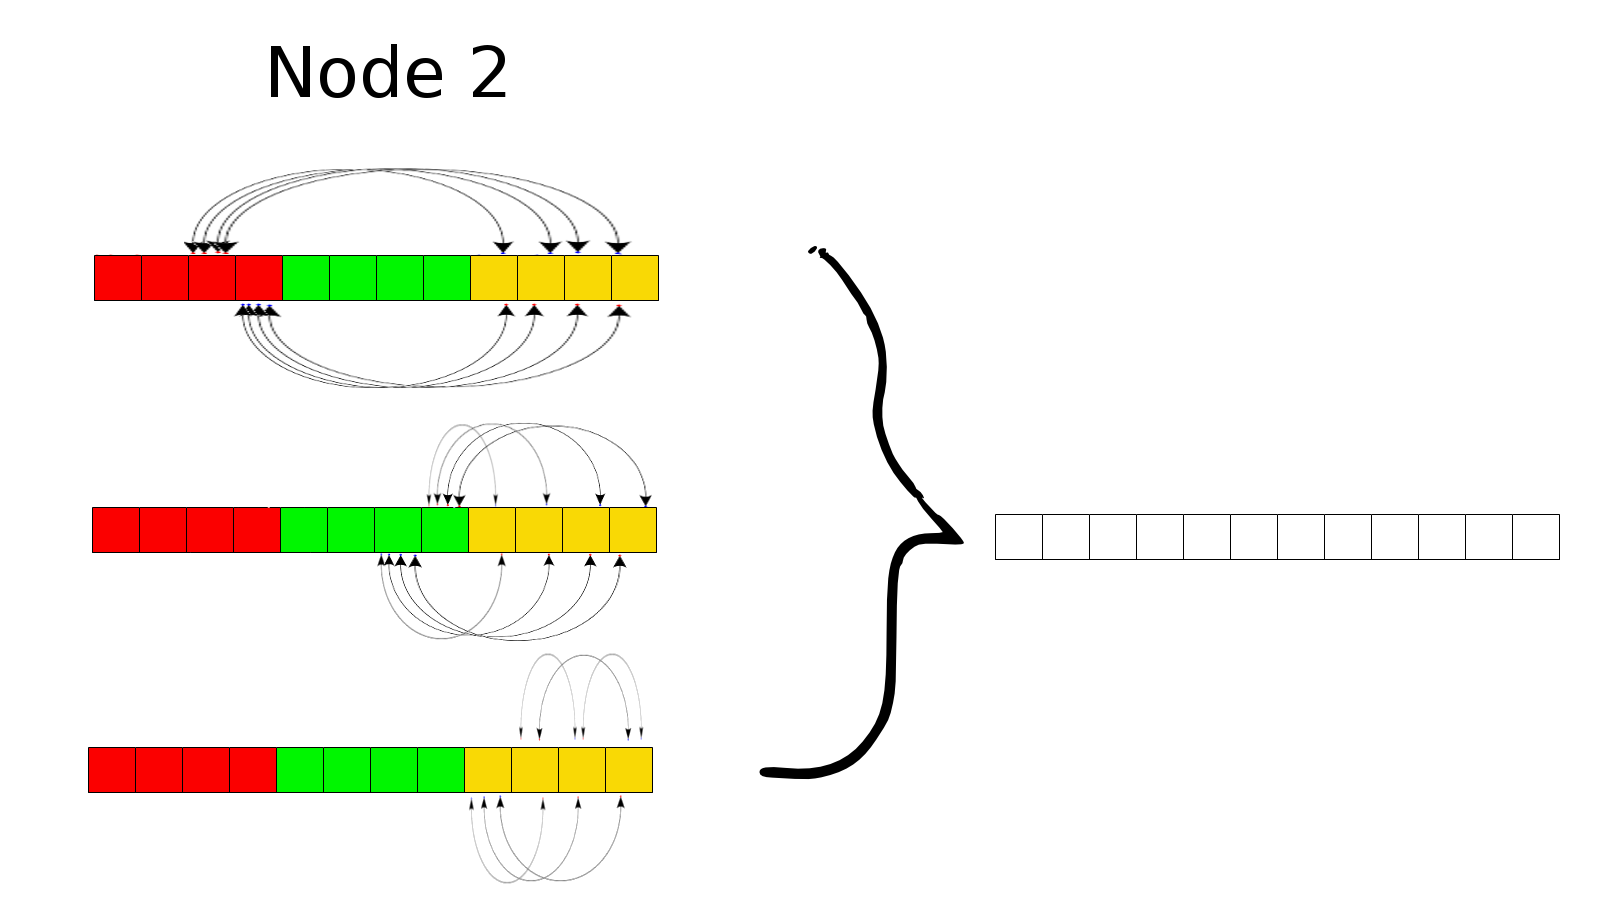
\includegraphics[width=0.5\linewidth]{force_calculation_2}
\end{subfigure}
  \caption{C - Forces computation, the results are put in a vector}
  \label{fig:C1}
\end{figure}
\FloatBarrier



\begin{figure}
\centering
\begin{minipage}{.45\textwidth}
  \centering
  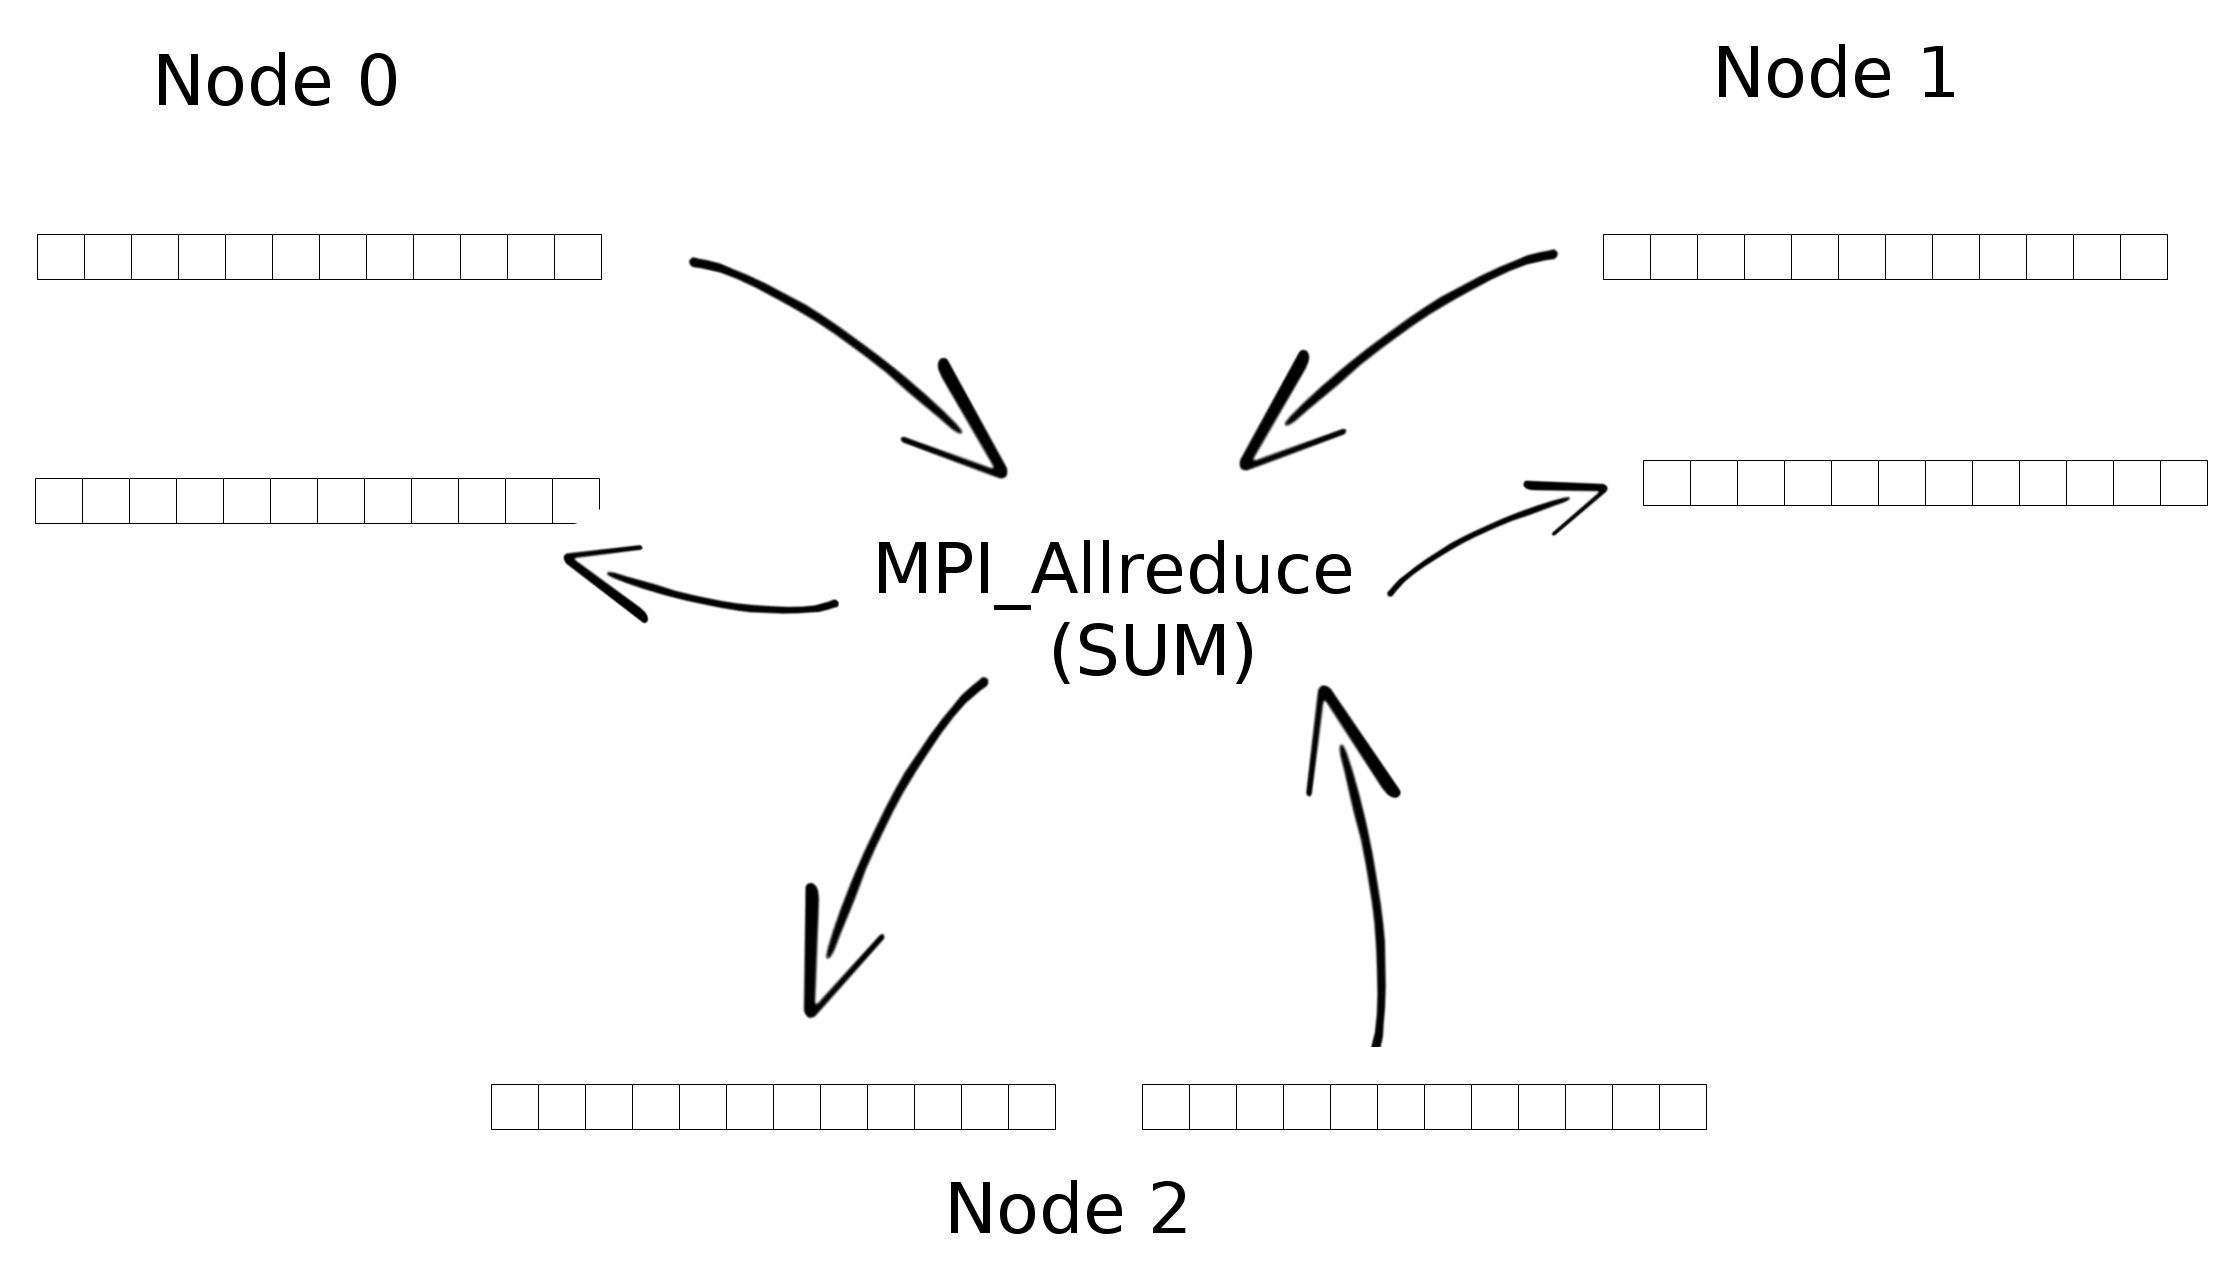
\includegraphics[width=1\linewidth]{MPI_all_reduce}
  \captionof{figure}{D - Forces reduction, sum all the vectors of forces calculated by different nodes}
  \label{fig:D1}
\end{minipage}%
\begin{minipage}{.45\textwidth}
  \centering
  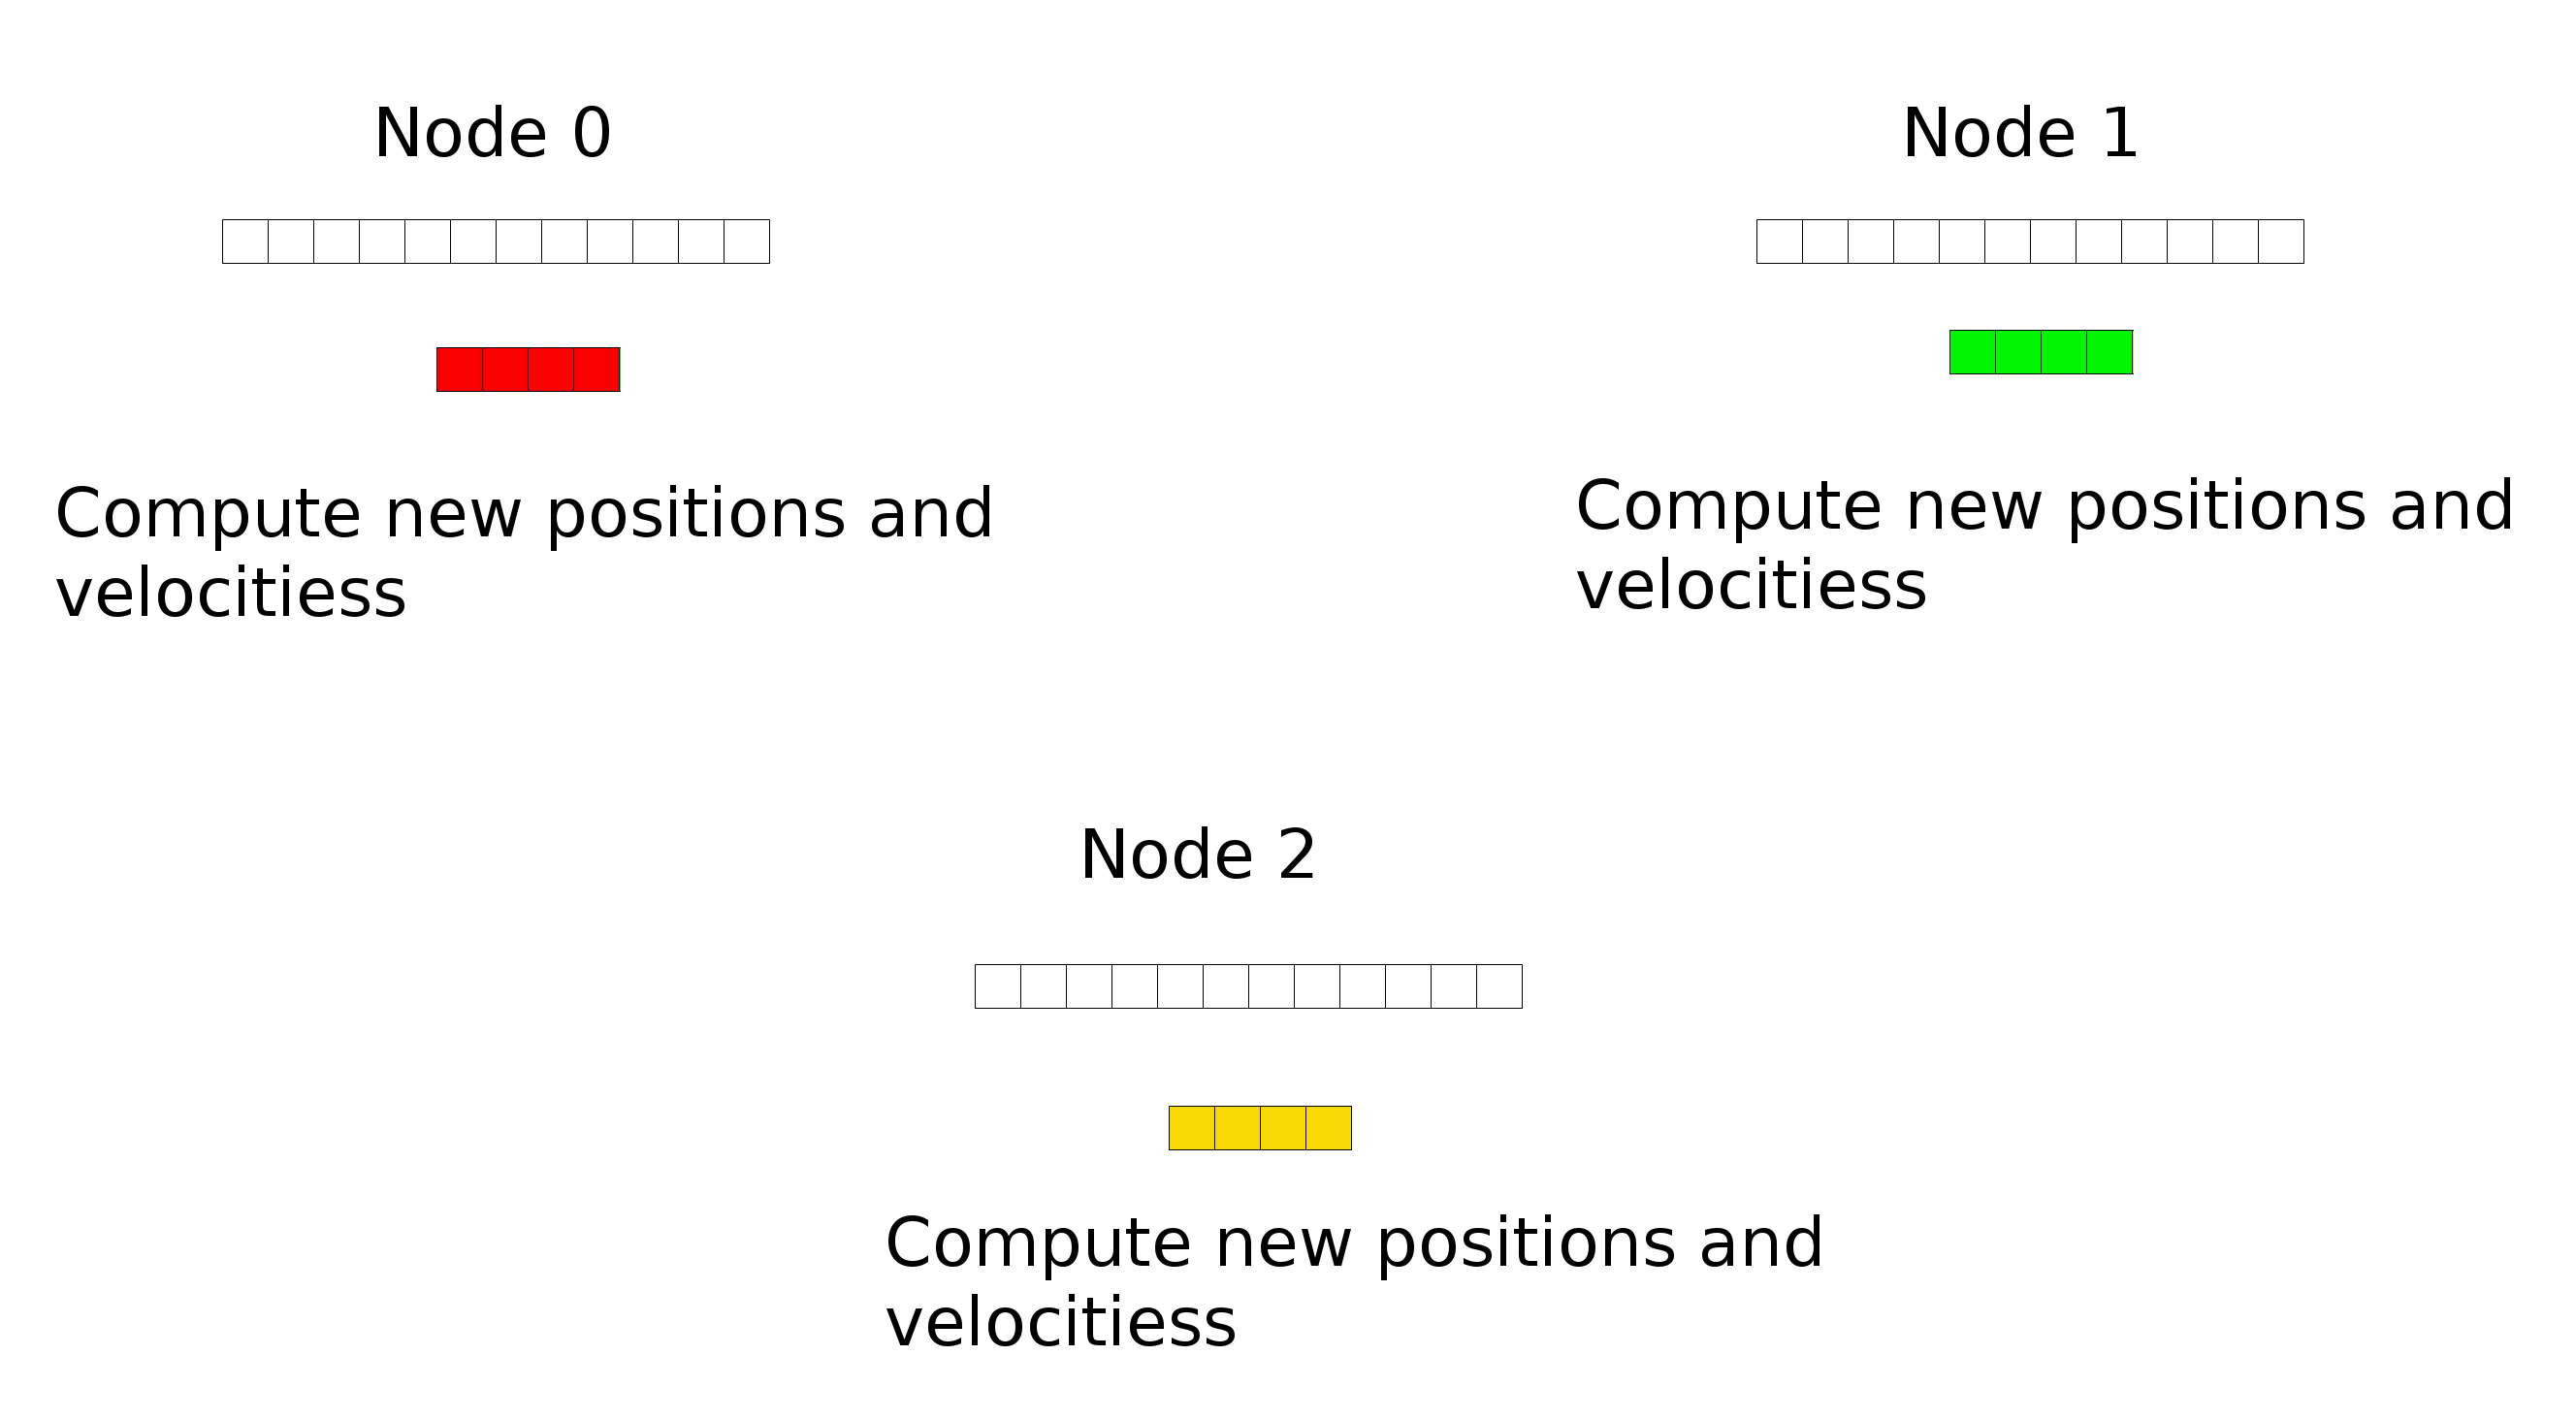
\includegraphics[width=1\linewidth]{compute_positions_only}
  \captionof{figure}{E - Update positions and velocities for bodies of the assigned chunk }
  \label{fig:E1}
\end{minipage}
\end{figure}
\FloatBarrier

\begin{equation} \label{eq:comp_app2}
\begin{split}
Complexity (per step) & = O(\lceil\frac{N^2}{2P}\rceil)) + O(\lceil\frac{N}{P}\rceil) + O(\lceil\frac{N}{P}\rceil)\\
 & = O(\lceil\frac{N^2}{2P}\rceil)
\end{split}
\end{equation}

\begin{equation} \label{eq:com_app2}
\begin{split}
Communication (per step) & = O(N)*sizeof(bodyType)
\end{split}
\end{equation}


\subsubsection{Solutions comparison}
\label{sec:sol_comp}
After a comparison of the two solutions for different size of inputs (steps and number of bodies), it's clear that the amount of data exchanged is the key point. In Tables \ref{tab:t_app1} and \ref{tab:t_app2} (corresponding graphs in Figure \ref{fig:G1}) and in Tables \ref{tab:t_app3} and \ref{tab:t_app4} (corresponding graphs in Figure \ref{fig:G2}) we can see execution times and speedups of the 2 approaches for different problem sizes. It's easy to understand that the first approach present lower execution times than the other and so better speedups. That means that is more convenient to compute the N velocities and positions in all the nodes inste ad of exchange more data with the other nodes. The first approach so is better.
\\


\begin{minipage}[b]{.40\textwidth}
  \centering
  \begin{tabular}{l|l|l}
  \centering
nodes\textbackslash approach & 1 & 2 \\ \hline
1 & 107.856 & 107.856 \\ \hline
2 & 63.612 & 83.450 \\ \hline
4 & 33.939 & 45.068 \\ \hline
8 & 19.566 & 26.229 \\ \hline
10 & 16.916 & 23.593 \\ \hline
16 & 12.584 & 17.523 \\ 
    \hline
  \end{tabular}
  \captionof{table}{128 bodies and 100000 iterations - Execution times}
  \label{tab:t_app1}
\end{minipage} \qquad
\begin{minipage}[b]{.40\textwidth}
  \centering
  \begin{tabular}{l|l|l}
nodes\textbackslash approach & 1 & 2 \\ \hline
2 & 1.69 & 1.29 \\ \hline
4 & 3.17 & 2.39 \\ \hline
8 & 5.51 & 4.11 \\ \hline
10 & 6.37 & 4.57 \\ \hline
16 & 8.57 & 6.15 \\ 
  \hline
  \end{tabular}
  \captionof{table}{128 bodies and 100000 iterations - Speedups}
  \label{tab:t_app2}
\end{minipage}

\begin{figure}[ht]
\begin{subfigure}{.55\textwidth}
  \centering
  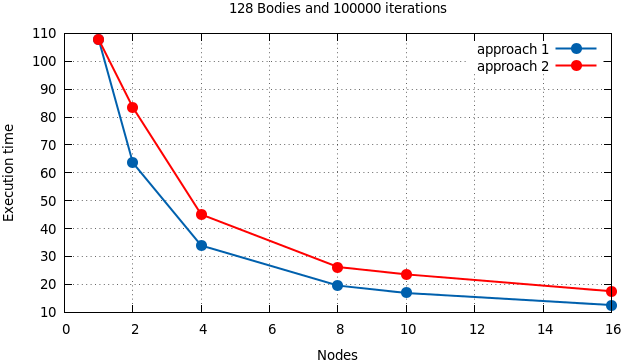
\includegraphics[width=1\linewidth]{results/graph1}
\end{subfigure} %
\begin{subfigure}{.35\textwidth}
  \centering
  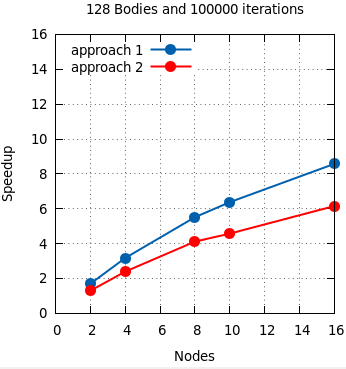
\includegraphics[width=1\linewidth]{results/graph1_sp}
\end{subfigure} 
  \caption{Execution Time and Speedups of the two approaches with 128 bodies and 100000 iterations}
  \label{fig:G1}
\end{figure}
\FloatBarrier


\enspace

\begin{minipage}[b]{.40\textwidth}
  \centering
  \begin{tabular}{l|l|l}
  \centering
nodes\textbackslash approach & 1 & 2 \\ \hline
1 & 655.162 & 655.162 \\ \hline
2 & 373.328 & 481.161 \\ \hline
4 & 186.764 & 240.538 \\ \hline
8 & 93.483 & 120.394 \\ \hline
10 & 74.908 & 96.431 \\ \hline
16 & 47.192 & 60.563 \\ 
    \hline
  \end{tabular}
  \captionof{table}{10000 bodies and 100 iterations - Execution times}
  \label{tab:t_app3}
\end{minipage} \qquad
\begin{minipage}[b]{.40\textwidth}
  \centering
  \begin{tabular}{l|l|l}
nodes\textbackslash approach & 1 & 2 \\ \hline
2 & 1.75 & 1.36 \\ \hline
4 & 3.5 & 2.72 \\ \hline
8 & 7 & 5.44 \\ \hline
10 & 8.74 & 6.79 \\ \hline
16 & 13.88 & 10.81 \\ 
  \hline
  \end{tabular}
  \captionof{table}{10000 bodies and 100 iterations - Speedups}
  \label{tab:t_app4}
\end{minipage}


\begin{figure}[ht]
\begin{subfigure}{.55\textwidth}
  \centering
  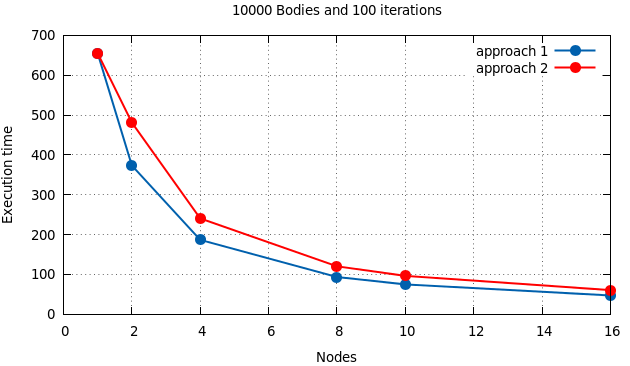
\includegraphics[width=1\linewidth]{results/graph2}
\end{subfigure} %
\begin{subfigure}{.35\textwidth}
  \centering
  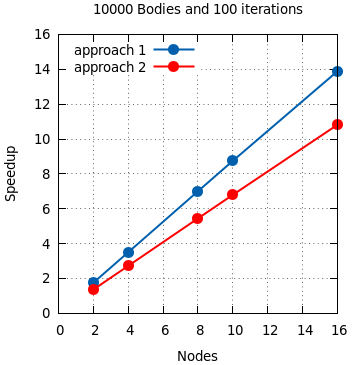
\includegraphics[width=1\linewidth]{results/graph2_sp}
\end{subfigure}
  \caption{Execution Time and Speedups of the two approaches with 10000 bodies and 100 iterations}
  \label{fig:G2}
\end{figure}
\FloatBarrier


\subsubsection{Results}
\label{sec:res}
In this section some obtained results are reported. In Figure \ref{fig:R1} and Tables \ref{tab:R1_t1}, \ref{tab:R1_t2} we have an example with a big number of iterations (fixed) and different numbers of bodies (small). In Figure \ref{fig:R2} and Tables \ref{tab:R2_t1}, \ref{tab:R2_t2} we have an example with a small number of iterations (fixed) and different numbers of bodies (big). As we can see, more we increase the size of the problem and more the implementation obtains good speedups. The aim of parallel programming is to deal with big size problems, so this implementation is good due to the fact that the more we increase the number of bodies, the more the speedup is close to be linear. \\

\begin{figure}[ht]
\begin{subfigure}{.5\textwidth}
  \centering
  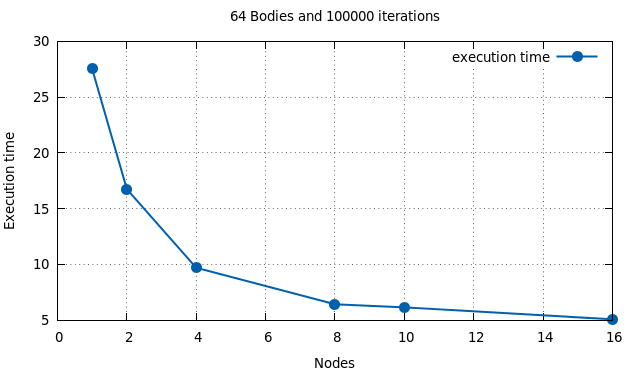
\includegraphics[width=1\linewidth]{results/graph3}
\end{subfigure} %
\begin{subfigure}{.5\textwidth}
  \centering
  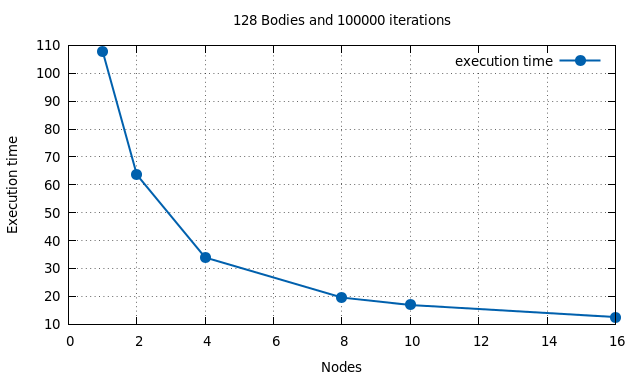
\includegraphics[width=1\linewidth]{results/graph4}
\end{subfigure} \\ %
\begin{subfigure}{.5\textwidth}
  \centering
  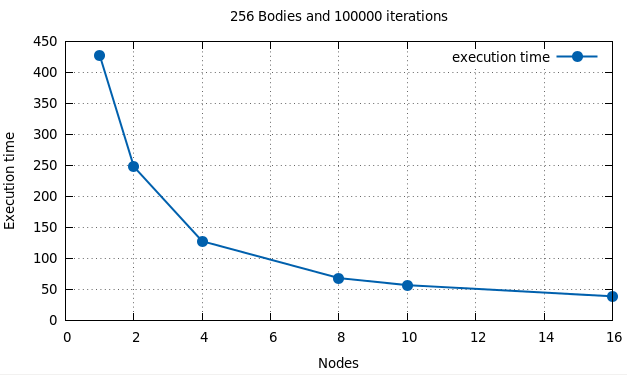
\includegraphics[width=1\linewidth]{results/graph5}
\end{subfigure} %
\begin{subfigure}{.4\textwidth}
  \centering
  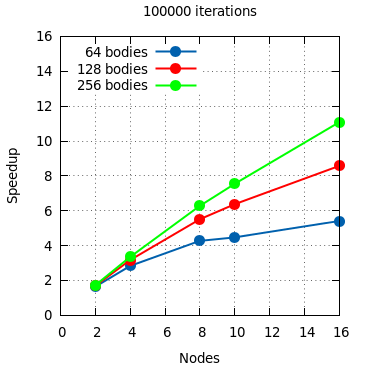
\includegraphics[width=1\linewidth]{results/graph5_sp}
\end{subfigure}
  \caption{Execution Time and Speedups, 100000 iterations}
  \label{fig:R1}
\end{figure}
\FloatBarrier

\enspace

\begin{minipage}[b]{.40\textwidth}
  \centering
  \begin{tabular}{l|l|l|l}
  \centering
nodes\textbackslash bodies & 64 & 128 & 256 \\ \hline
1 & 27.533 & 107.856 & 427.855 \\ \hline
2 & 16.752 & 63.612 & 247.778 \\ \hline
4 & 9.706 & 33.939 & 127.529 \\ \hline
8 & 6.435 & 19.566 & 68.082 \\ \hline
10 & 6.155 & 16.916 & 56.687 \\ \hline
16 & 5.081 & 12.584 & 38.576 \\ 
    \hline
  \end{tabular}
  \captionof{table}{100000 iterations - Exec. times}
  \label{tab:R1_t1}
\end{minipage} \qquad
\begin{minipage}[b]{.40\textwidth}
  \centering
  \begin{tabular}{l|l|l|l}
nodes\textbackslash bodies & 64 & 128 & 256 \\ \hline
2 & 1.64 & 1.69 & 1.72 \\ \hline
4 & 2.83 & 3.17 & 3.35 \\ \hline
8 & 4.27 & 5.51 & 6.28 \\ \hline
10 & 4.47 & 6.37 & 7.54 \\ \hline
16 & 5.41 & 8.57 & 11.08 \\ 
  \hline
  \end{tabular}
  \captionof{table}{100000 iterations - Speedups}
  \label{tab:R1_t2}
\end{minipage}

\begin{figure}[ht]
\begin{subfigure}{.5\textwidth}
  \centering
  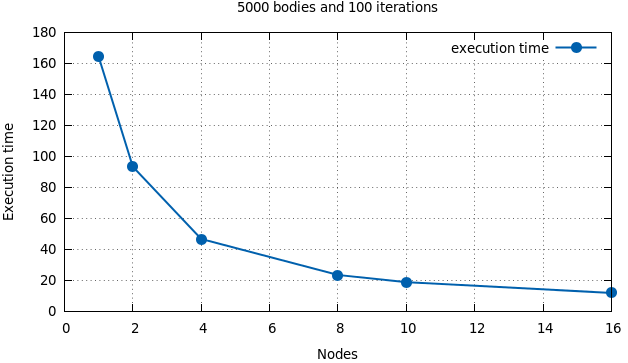
\includegraphics[width=1\linewidth]{results/graph11}
\end{subfigure} %
\begin{subfigure}{.5\textwidth}
  \centering
  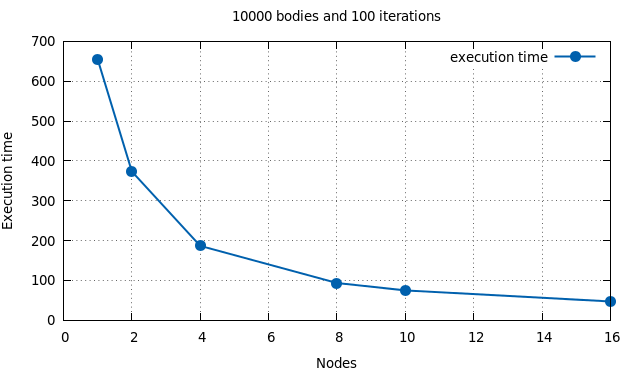
\includegraphics[width=1\linewidth]{results/graph14}
\end{subfigure} \\ %
\begin{subfigure}{.5\textwidth}
  \centering
  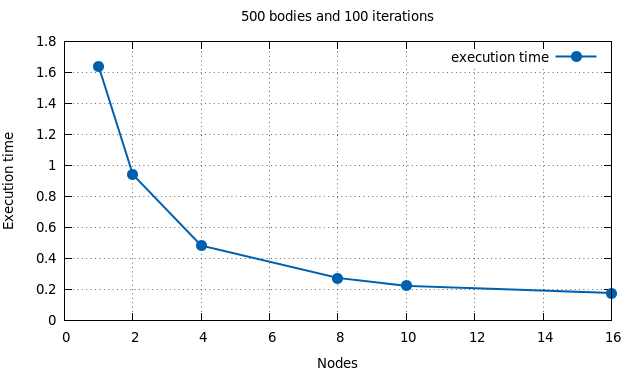
\includegraphics[width=1\linewidth]{results/graph15}
\end{subfigure} %
\begin{subfigure}{.5\textwidth}
  \centering
  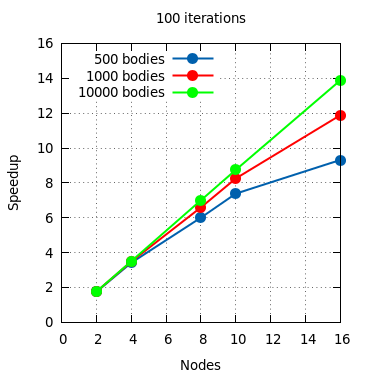
\includegraphics[width=1\linewidth]{results/graph16}
\end{subfigure} 
  \caption{Execution Time and Speedups, 100 iterations}
  \label{fig:R2}
\end{figure}
\FloatBarrier

\begin{minipage}[b]{.40\textwidth}
  \centering
  \begin{tabular}{l|l|l|l}
  \centering
nodes\textbackslash bodies & 500 & 1000 & 10000 \\ \hline
1 & 1.639 & 6.598 & 655.162 \\ \hline
2 & 0.940 & 3.749 & 373.328 \\ \hline
4 & 0.482 & 1.892 & 186.764 \\ \hline
8 & 0.273 & 1.001 & 93.483 \\ \hline
10 & 0.222 & 0.799 & 74.908 \\ \hline
16 & 0.176 & 0.555 & 47.192 \\ 
    \hline
  \end{tabular}
  \captionof{table}{100000 iterations - Exec. times}
  \label{tab:R2_t1}
\end{minipage} \qquad
\begin{minipage}[b]{.40\textwidth}
  \centering
  \begin{tabular}{l|l|l|l}
nodes\textbackslash bodies & 500 & 1000 & 10000 \\ \hline
2 & 1.74 & 1.75 & 1.75 \\ \hline
4 & 3.41 & 3.48 & 3.5 \\ \hline
8 & 6 & 6.59 & 7 \\ \hline
10 & 7.38 & 8.25 & 8.74 \\ \hline
16 & 9.31 & 11.88 & 13.88 \\ 
  \hline
  \end{tabular}
  \captionof{table}{100000 iterations - Speedups}
  \label{tab:R2_t2}
\end{minipage}	


As expected, if we fix the number of bodies and we change the number of iterations, we obtain the same speedup results (Figure \ref{fig:R3} and Tables \ref{tab:R3_t1}, \ref{tab:R3_t2}). This is due to the fact that we have to repeat the same work but different times.

\begin{figure}[ht]
\begin{subfigure}{.5\textwidth}
  \centering
  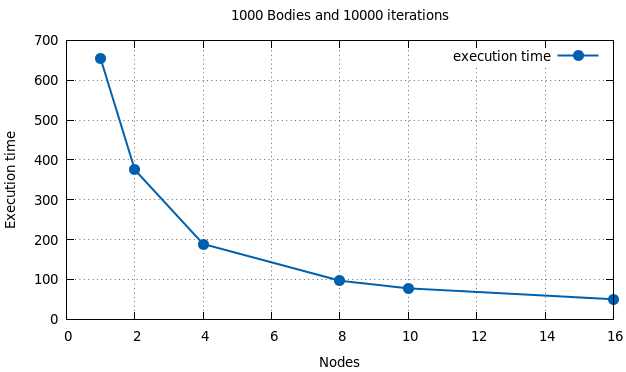
\includegraphics[width=1\linewidth]{results/graph19}
\end{subfigure} %
\begin{subfigure}{.5\textwidth}
  \centering
  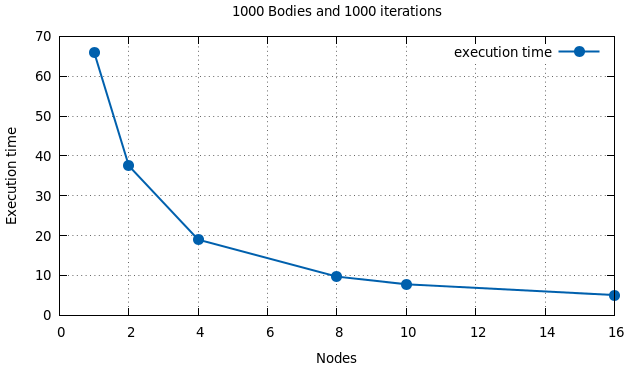
\includegraphics[width=1\linewidth]{results/graph17}
\end{subfigure} \\ %
\begin{subfigure}{\textwidth}
  \centering
  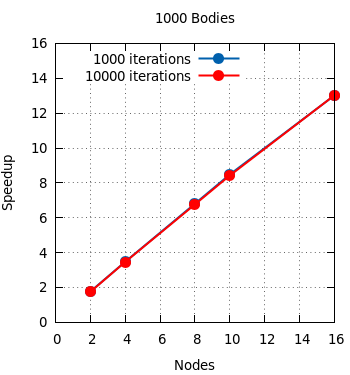
\includegraphics[width=.4\linewidth]{results/graph18}
\end{subfigure} 
  \caption{Execution Time and Speedups, 1000 bodies}
  \label{fig:R3}
\end{figure}
\FloatBarrier


\begin{minipage}[b]{.40\textwidth}
  \centering
  \begin{tabular}{l|l|l}
  \centering
nodes\textbackslash iterations & 1000 & 10000 \\ \hline
1 & 65.991 & 654.008 \\ \hline
2 & 37.488 & 374.935 \\ \hline
4 & 18.989 & 188.824 \\ \hline
8 & 9.702 & 96.724 \\ \hline
10 & 7.778 & 77.597 \\ \hline
16 & 5.070 & 50.201 \\ 
    \hline
  \end{tabular}
  \captionof{table}{1000 bodies - Execution times}
  \label{tab:R3_t1}
\end{minipage} \qquad
\begin{minipage}[b]{.40\textwidth}
  \centering
  \begin{tabular}{l|l|l}
nodes\textbackslash iterations & 1000 & 10000 \\ \hline
2 & 1.76 & 1.74 \\ \hline
4 & 3.47 & 3.46 \\ \hline
8 & 6.8 & 6.76 \\ \hline
10 & 8.48 & 8.42 \\ \hline
16 & 13.01 & 13.02 \\ 
  \hline
  \end{tabular}
  \captionof{table}{1000 bodies - Speedups}
  \label{tab:R3_t2}
\end{minipage}	

All the tests were performed on the Leiden University cluster (fs1.das4.liacs.nl) and the execution times were measured using the "wall clock time". Data distribution and data gathering (as being part of the application's initialisation and de-initialisation) are not considered on the measured performance.

\section{Conclusions and Personal considerations}
\label{sec:con}
With the realized implementation, the speedups are close to be linear for big size problems and that means that is a good implementation. This was the first time for me to use the MPI programming model and the hardest part was to understand how the MPI operations work and use them to compute various tests (e.g. MPI\_Allgatherv, MPI\_Scatterv). From my work I understood the powerful of this programming model and that is interesting to have more than one implementation in order to compare the results and outline any weaknesses.  

		
\printbibliography 

\end{document}